\subsection{Progettazione e Codifica}

\subsubsection{I Incremento}
\subsubsubsection{Prospetto orario}
In questo incremento la distribuzione oraria è la seguente:
\begin{table}[H]
\begin{center}
\rowcolors{2}{gray!25}{white}
\renewcommand{\arraystretch}{1.25}
\begin{tabular}{ m{0.20\textwidth}<{\centering}  m{0.06\textwidth}<{\centering} m{0.06\textwidth}<{\centering} m{0.06\textwidth}<{\centering}  m{0.06\textwidth}<{\centering}  m{0.06\textwidth}<{\centering}  m{0.06\textwidth}<{\centering}  m{0.20\textwidth}<{\centering}   }
	\rowcolor{darkblue}
	\textcolor{white}{\textbf{Componente}} &\textcolor{white}{\textbf{Re}}&\textcolor{white}{\textbf{Pt}}&\textcolor{white}{\textbf{An}}&\textcolor{white}{\textbf{Am}}&\textcolor{white}{\textbf{Pr}}&\textcolor{white}{\textbf{Ve}}&\textcolor{white}{\textbf{Ore complessive}}\\ 
	Edoardo Pavan & 1 & 0 & 0 & 1 & 0 & 1 & 3 \\	
	
	Francesco Protopapa & 0 & 1 & 0 & 0 & 0 & 2 & 3 \\

	Greta Cavedon & 0 & 1 & 0 & 0 & 1 & 1 & 3 \\
	
	Luciano Wu & 1 & 1 & 0 & 0 & 1 & 0 & 3 \\
	
	Matteo Basso & 0 & 1 & 1 & 0 & 2 & 1 & 5 \\
	
	Michele Gatto & 2 & 0 & 0 & 0 & 0 & 1 & 3 \\
	
	Pietro Villatora & 0 & 1 & 0 & 1 & 0 & 0 & 2 \\
	
	\textbf{Ore totali ruolo} & 4 & 5 & 1 & 2 & 4 & 6 & 22 \\

\end{tabular}
\caption{Distribuzione oraria per ogni componente nel I incremento di Progettazione e Codifica}
\end{center}
\end{table}

La tabella può essere rappresentata anche in forma visiva dal seguente grafico:
\begin{figure}[H]
\centering
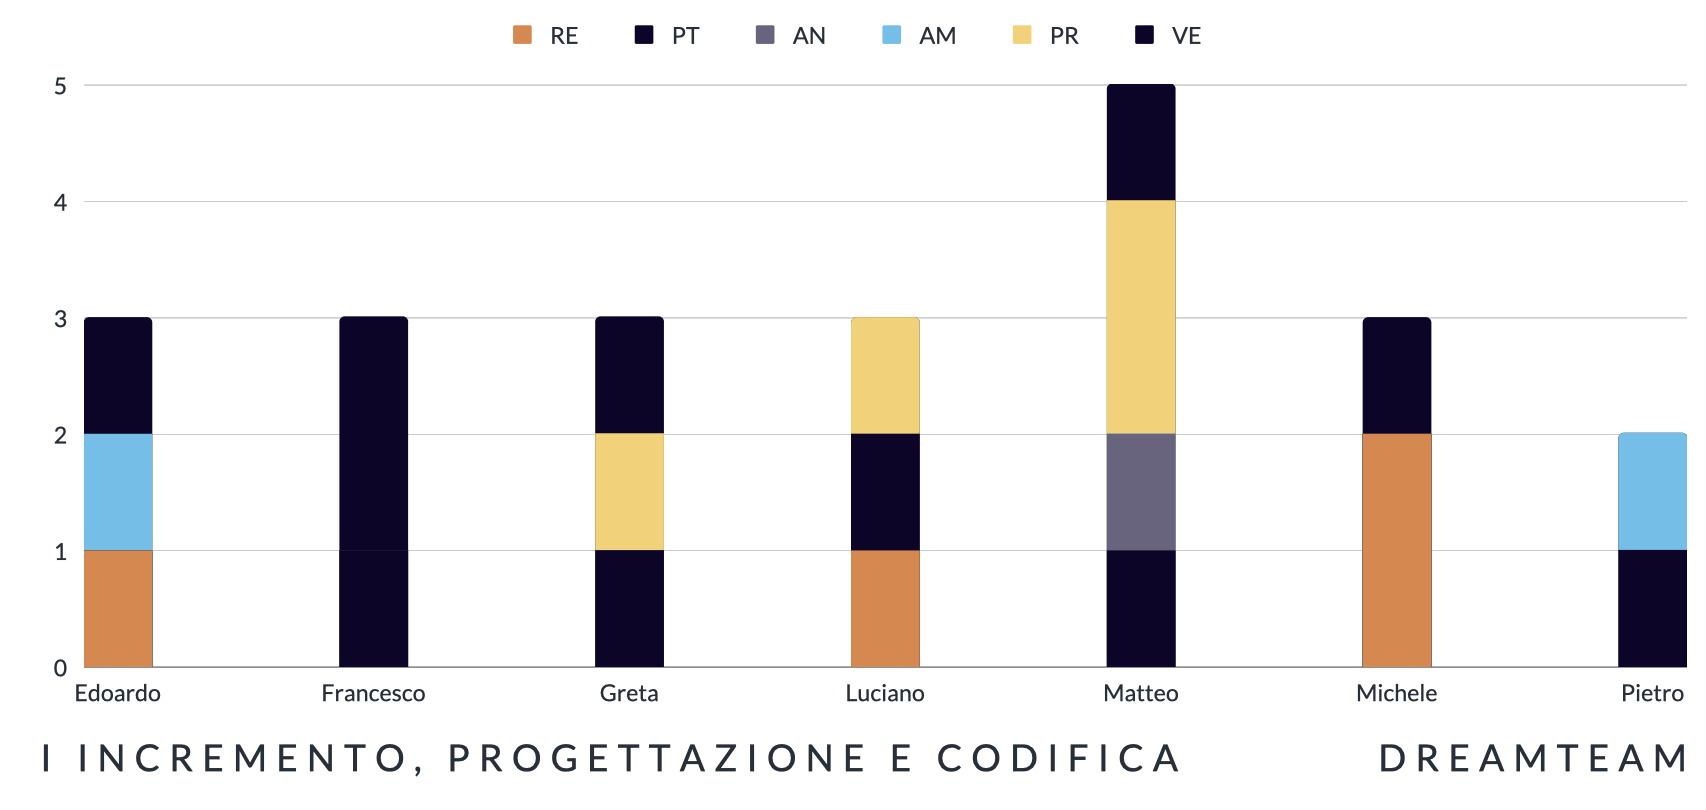
\includegraphics[scale=0.50]{Sezioni/SezioniPreventivo/grafici/progettazione/Progettazione_I_incremento.png}
\caption{Istogramma della ripartizione delle ore nel I incremento di Progettazione e Codifica}
\end{figure}

\subsubsubsection{Prospetto economico}
La seguente tabella rappresenta le ore totali dedicate ad ogni ruolo e il costo in euro:

\begin{table}[H]
\begin{center}
\rowcolors{2}{gray!25}{white}
\renewcommand{\arraystretch}{1.5}
\begin{tabular}{ m{0.3\textwidth}<{\centering}  m{0.2\textwidth}<{\centering} m{0.2\textwidth}<{\centering}}
	\rowcolor{darkblue}
	\textcolor{white}{\textbf{Ruolo}}&\textcolor{white}{\textbf{Totale ore}}&\textcolor{white}{\textbf{Costo totale (\euro)}}\\ 

	Responsabile  & 4 & 120 \\	
	
	Progettista & 5 & 125 \\
	
	Analista & 1 & 25 \\

	Amministratore & 2 & 40 \\
	
	Programmatore & 4 & 60 \\
	
	Verificatore & 6 & 90 \\
	
	\textbf{Totale} & 22 & 460 \\
	
\end{tabular}
\caption{Prospetto dei costi per ruolo nel I incremento di Progettazione e Codifica}
\end{center}
\end{table}

La tabella può essere rappresentata anche in forma visiva dal seguente aerogramma:
\begin{figure}[H]
\centering
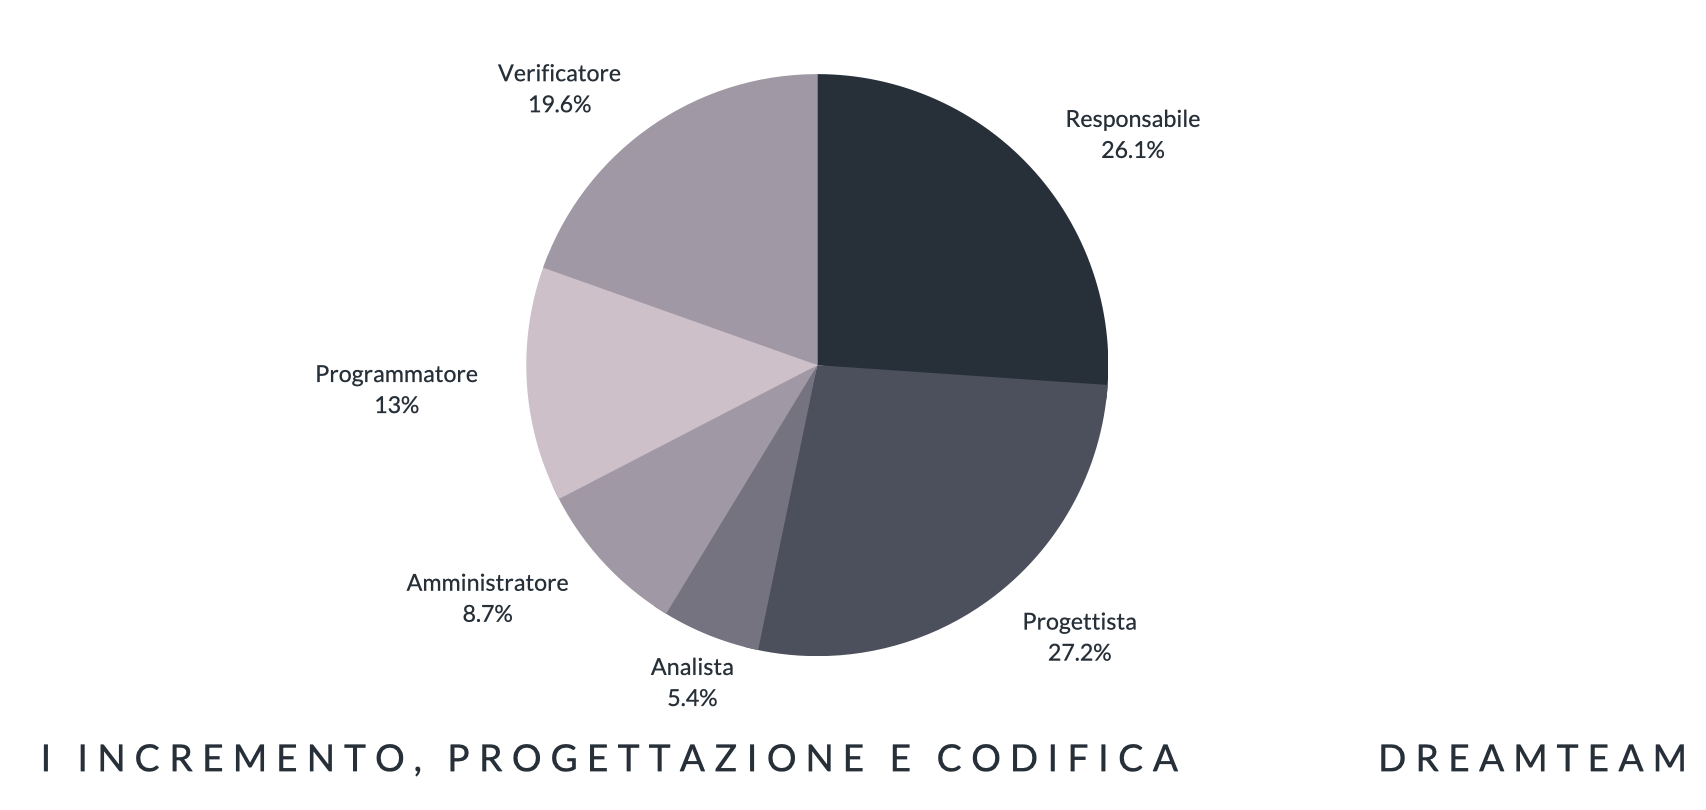
\includegraphics[scale=0.50]{Sezioni/SezioniPreventivo/grafici/progettazione/Progettazione_I_incremento_costi.png}
\caption{Grafico a torta della ripartizione per ruolo delle ore durante il I incremento di Progettazione e Codifica}
\end{figure}

\pagebreak

\subsubsection{II Incremento}
\subsubsubsection{Prospetto orario}
In questa incremento la distribuzione oraria è la seguente:
\begin{table}[H]
\begin{center}
\rowcolors{2}{gray!25}{white}
\renewcommand{\arraystretch}{1.25}
\begin{tabular}{ m{0.20\textwidth}<{\centering}  m{0.06\textwidth}<{\centering} m{0.06\textwidth}<{\centering} m{0.06\textwidth}<{\centering}  m{0.06\textwidth}<{\centering}  m{0.06\textwidth}<{\centering}  m{0.06\textwidth}<{\centering}  m{0.20\textwidth}<{\centering}   }
	\rowcolor{darkblue}
	\textcolor{white}{\textbf{Componente}} &\textcolor{white}{\textbf{Re}}&\textcolor{white}{\textbf{Pt}}&\textcolor{white}{\textbf{An}}&\textcolor{white}{\textbf{Am}}&\textcolor{white}{\textbf{Pr}}&\textcolor{white}{\textbf{Ve}}&\textcolor{white}{\textbf{Ore complessive}}\\ 
	Edoardo Pavan & 1 & 3 & 0 & 1 & 3 & 2 & 10 \\	
	
	Francesco Protopapa & 0 & 2 & 0 & 0 & 1 & 2 & 5 \\

	Greta Cavedon & 0 & 1 & 0 & 0 & 1 & 1 & 3 \\
	
	Luciano Wu & 1 & 1 & 0 & 1 & 2 & 0 & 5 \\
	
	Matteo Basso & 0 & 2 & 1 & 0 & 4 & 1 & 8 \\
	
	Michele Gatto & 1 & 1 & 0 & 0 & 2 & 1 & 5 \\
	
	Pietro Villatora & 0 & 2 & 0 & 0 & 5 & 1 & 8 \\
	
	\textbf{Ore totali ruolo} & 3 & 12 & 1 & 2 & 18 & 8 & 44 \\

\end{tabular}
\caption{Distribuzione oraria per ogni componente nel II incremento di Progettazione e Codifica}
\end{center}
\end{table}

La tabella può essere rappresentata anche in forma visiva dal seguente grafico:
\begin{figure}[H]
\centering
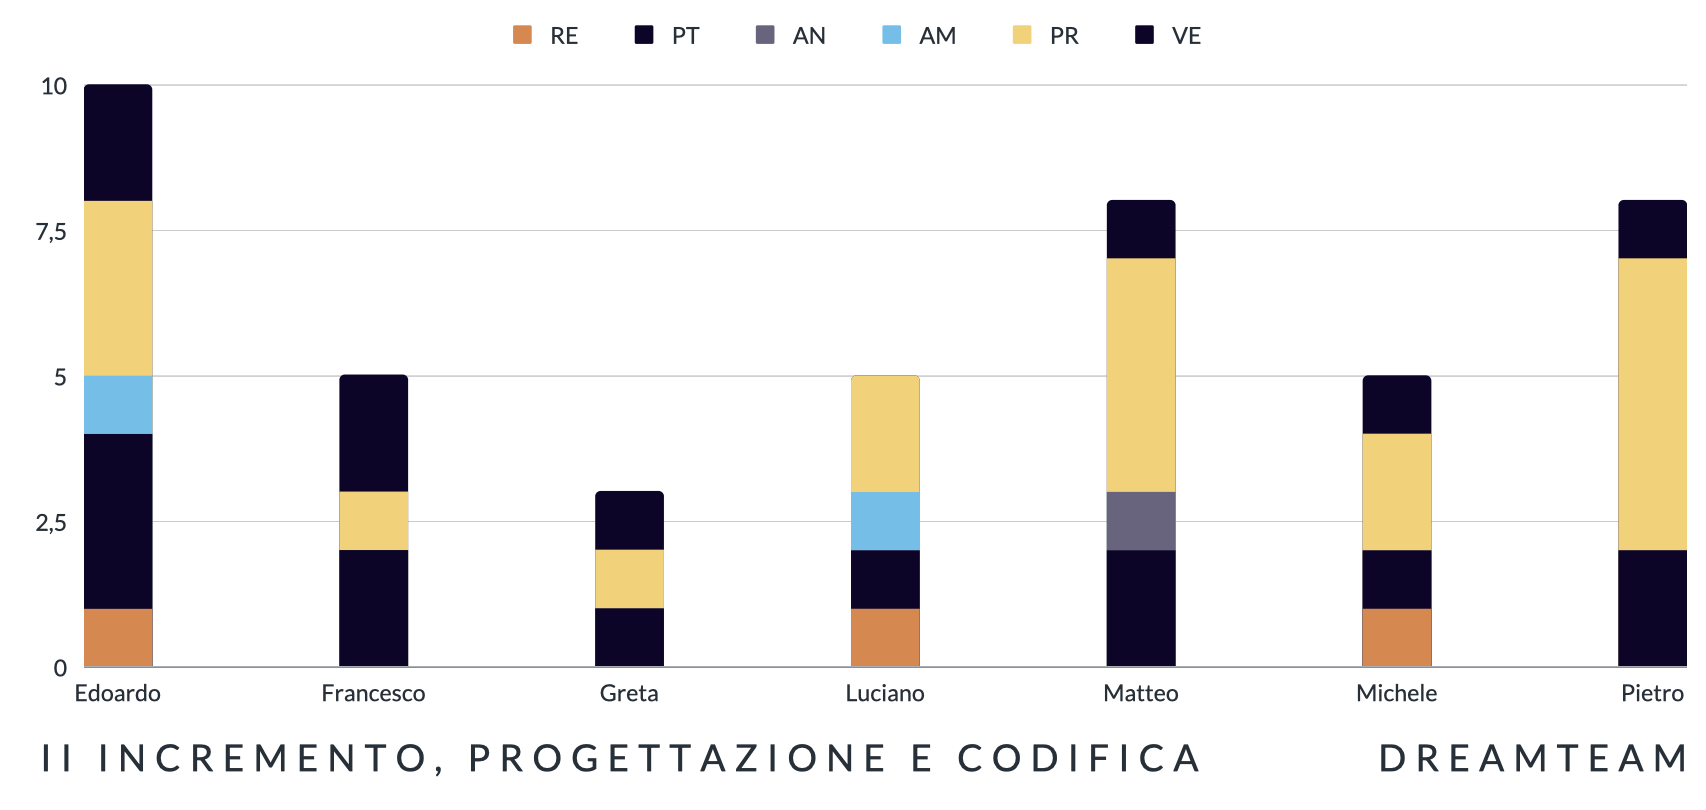
\includegraphics[scale=0.50]{Sezioni/SezioniPreventivo/grafici/progettazione/Progettazione_II_incremento.png}
\caption{Istogramma della ripartizione delle ore nel II incremento di Progettazione e Codifica}
\end{figure}

\subsubsubsection{Prospetto economico}
La seguente tabella rappresenta le ore totali dedicate ad ogni ruolo e il costo in euro:

\begin{table}[H]
\begin{center}
\rowcolors{2}{gray!25}{white}
\renewcommand{\arraystretch}{1.5}
\begin{tabular}{ m{0.3\textwidth}<{\centering}  m{0.2\textwidth}<{\centering} m{0.2\textwidth}<{\centering}}
	\rowcolor{darkblue}
	\textcolor{white}{\textbf{Ruolo}}&\textcolor{white}{\textbf{Totale ore}}&\textcolor{white}{\textbf{Costo totale (\euro)}}\\ 

	Responsabile & 3 & 90 \\	
	
	Progettista & 12 & 300 \\
	
	Analista & 1 & 25 \\

	Amministratore & 2 & 40 \\
	
	Programmatore & 18 & 270 \\
	
	Verificatore & 8 & 120 \\
	
	\textbf{Totale} & 44 & 845 \\
	
\end{tabular}
\caption{Prospetto dei costi per ruolo nel II incremento di Progettazione e Codifica}
\end{center}
\end{table}

La tabella può essere rappresentata anche in forma visiva dal seguente aerogramma:
\begin{figure}[H]
\centering
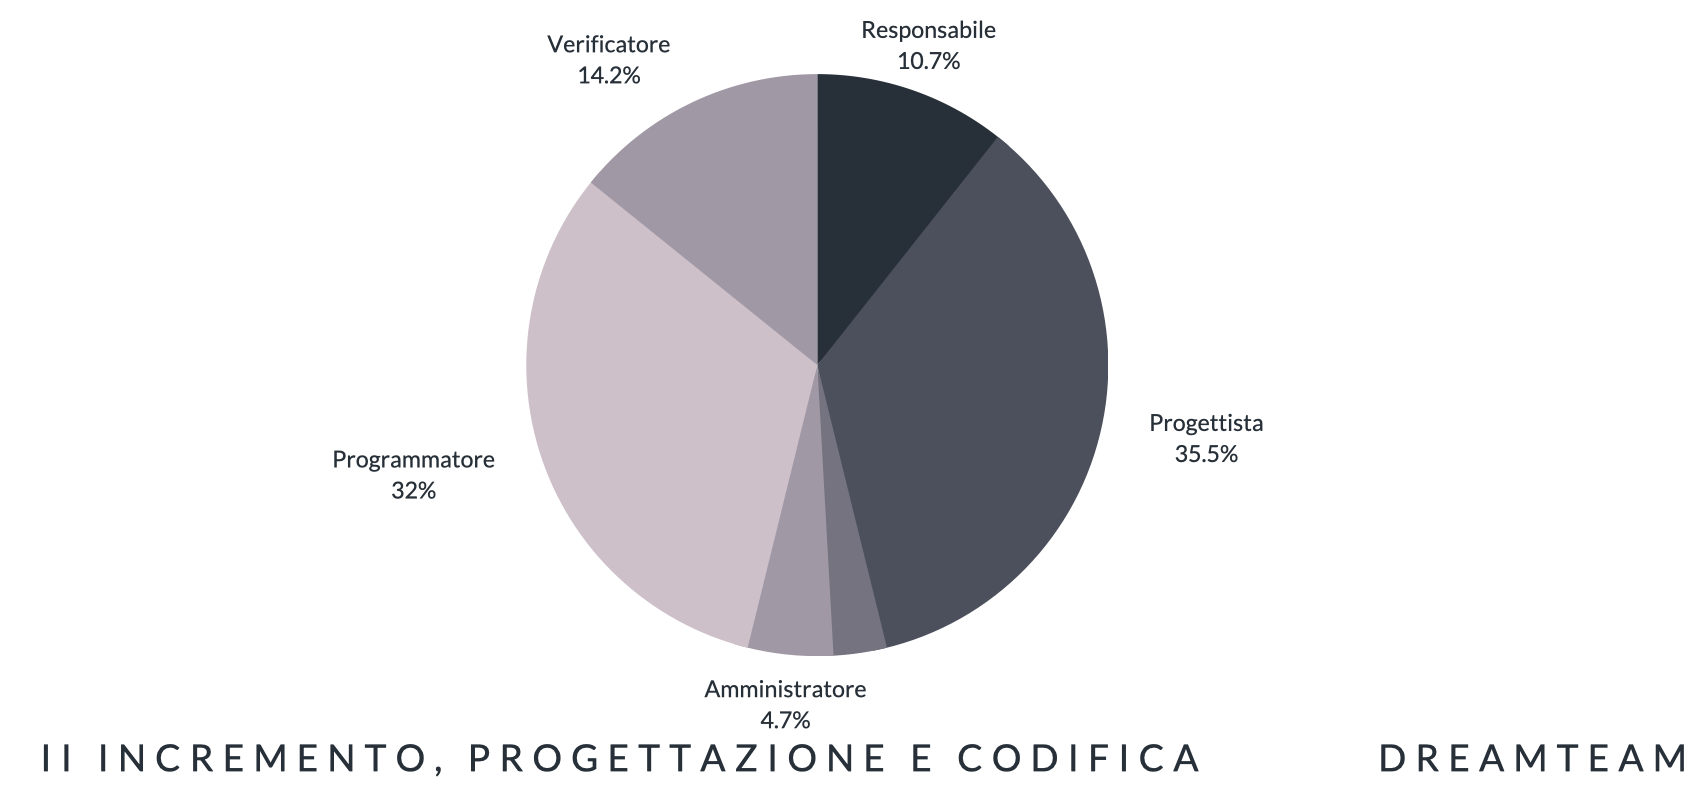
\includegraphics[scale=0.50]{Sezioni/SezioniPreventivo/grafici/progettazione/Progettazione_II_incremento_costi.png}
\caption{Grafico a torta della ripartizione per ruolo delle ore durante il II incremento di Progettazione e Codifica}
\end{figure}

\pagebreak


\subsubsection{III Incremento}
\subsubsubsection{Prospetto orario}
In questa fase la distribuzione oraria è la seguente:
\begin{table}[H]
\begin{center}
\rowcolors{2}{gray!25}{white}
\renewcommand{\arraystretch}{1.25}
\begin{tabular}{ m{0.20\textwidth}<{\centering}  m{0.06\textwidth}<{\centering} m{0.06\textwidth}<{\centering} m{0.06\textwidth}<{\centering}  m{0.06\textwidth}<{\centering}  m{0.06\textwidth}<{\centering}  m{0.06\textwidth}<{\centering}  m{0.20\textwidth}<{\centering}   }
	\rowcolor{darkblue}
	\textcolor{white}{\textbf{Componente}} &\textcolor{white}{\textbf{Re}}&\textcolor{white}{\textbf{Pt}}&\textcolor{white}{\textbf{An}}&\textcolor{white}{\textbf{Am}}&\textcolor{white}{\textbf{Pr}}&\textcolor{white}{\textbf{Ve}}&\textcolor{white}{\textbf{Ore complessive}}\\ 
	Edoardo Pavan & 0 & 2 & 0 & 1 & 3 & 1 & 7 \\	
	
	Francesco Protopapa & 1 & 1 & 0 & 0 & 3 & 0 & 5 \\

	Greta Cavedon & 1 & 1 & 0 & 0 & 3 & 1 & 6 \\
	
	Luciano Wu & 0 & 1 & 0 & 1 & 4 & 1 & 7 \\
	
	Matteo Basso & 0 & 2 & 2 & 0 & 4 & 1 & 9 \\
	
	Michele Gatto & 0 & 2 & 0 & 0 & 5 & 2 & 9 \\
	
	Pietro Villatora & 0 & 1 & 0 & 0 & 5 & 1 & 7 \\
	
	\textbf{Ore totali ruolo} & 2 & 10 & 2 & 2 & 27 & 7 & 50 \\

\end{tabular}
\caption{Distribuzione oraria per ogni componente nel III incremento di Progettazione e Codifica}
\end{center}
\end{table}

La tabella può essere rappresentata anche in forma visiva dal seguente grafico:
\begin{figure}[H]
\centering
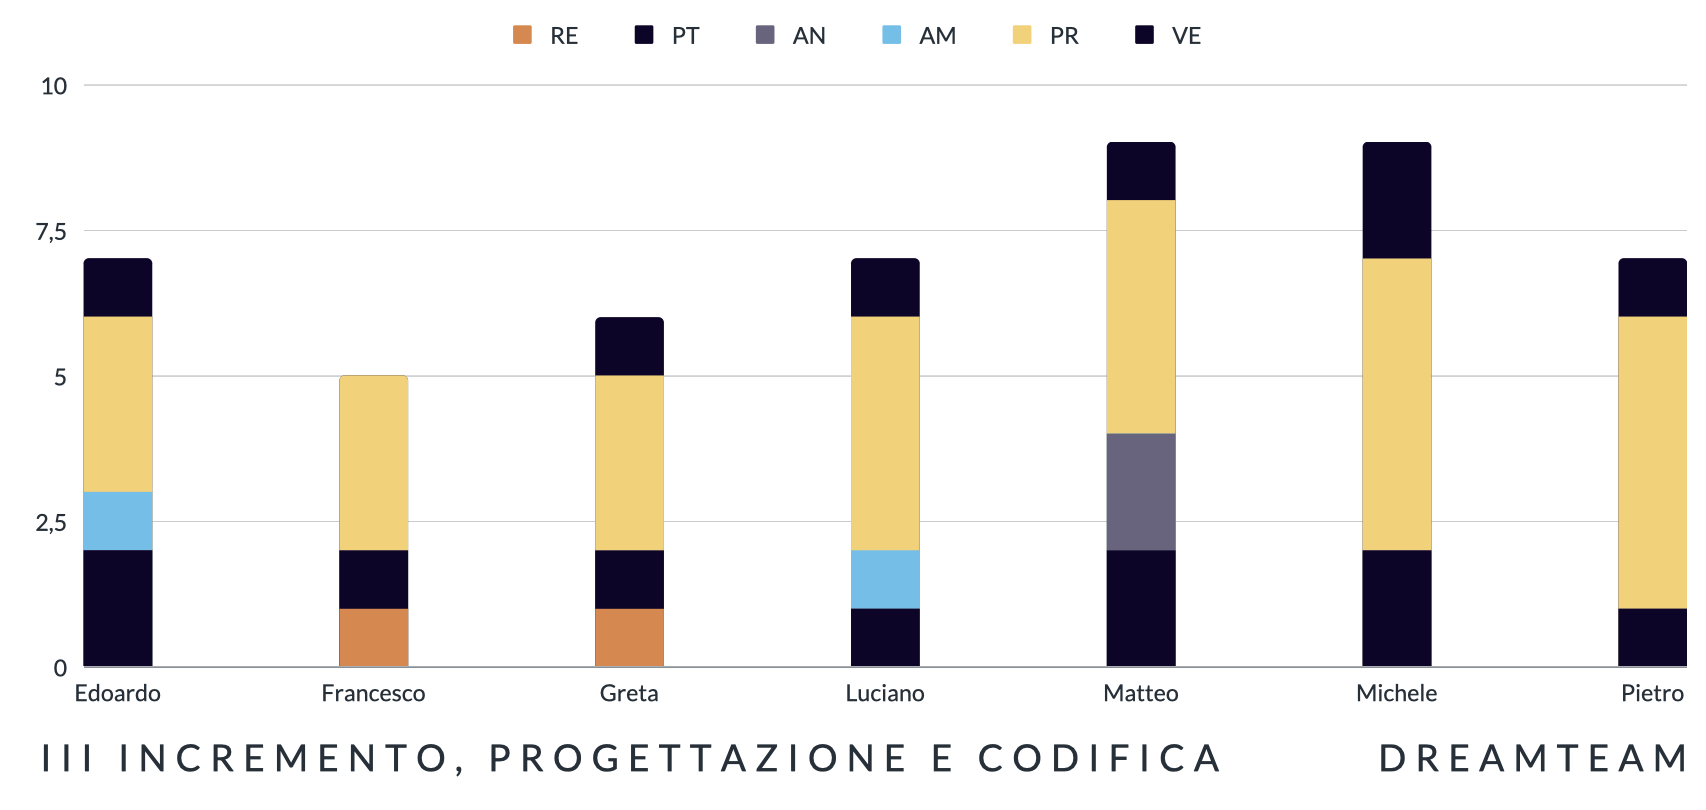
\includegraphics[scale=0.50]{Sezioni/SezioniPreventivo/grafici/progettazione/Progettazione_III_incremento.png}
\caption{Istogramma della ripartizione delle ore nel III incremento di Progettazione e Codifica}
\end{figure}

\subsubsubsection{Prospetto economico}
La seguente tabella rappresenta le ore totali dedicate ad ogni ruolo e il costo in euro:

\begin{table}[H]
\begin{center}
\rowcolors{2}{gray!25}{white}
\renewcommand{\arraystretch}{1.5}
\begin{tabular}{ m{0.3\textwidth}<{\centering}  m{0.2\textwidth}<{\centering} m{0.2\textwidth}<{\centering}}
	\rowcolor{darkblue}
	\textcolor{white}{\textbf{Ruolo}}&\textcolor{white}{\textbf{Totale ore}}&\textcolor{white}{\textbf{Costo totale (\euro)}}\\ 

	Responsabile  & 2 & 60 \\	
	
	Progettista & 10 & 250 \\
	
	Analista & 2 & 50 \\

	Amministratore & 2 & 40 \\
	
	Programmatore & 27 & 405 \\
	
	Verificatore & 7 & 105 \\
	
	\textbf{Totale} & 50 & 910 \\
	
\end{tabular}
\caption{Prospetto dei costi per ruolo nel III incremento di Progettazione e Codifica}
\end{center}
\end{table}

La tabella può essere rappresentata anche in forma visiva dal seguente aerogramma:
\begin{figure}[H]
\centering
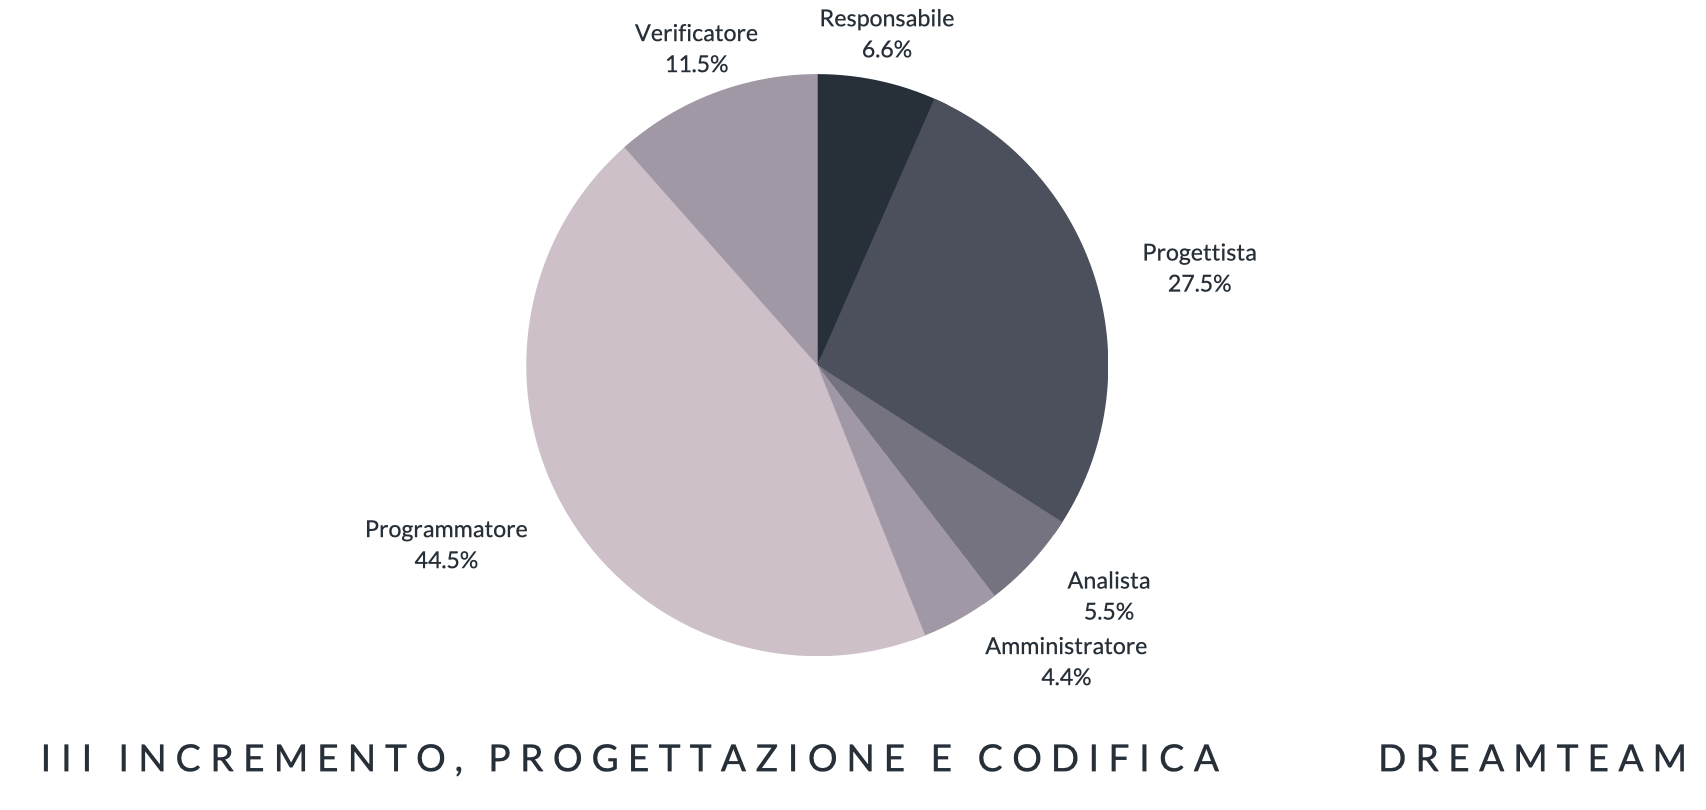
\includegraphics[scale=0.50]{Sezioni/SezioniPreventivo/grafici/progettazione/Progettazione_III_incremento_costi.png}
\caption{Grafico a torta della ripartizione per ruolo delle ore durante il III incremento di Progettazione e Codifica}
\end{figure}

\pagebreak


\subsubsection{IV Incremento}
\subsubsubsection{Prospetto orario}
In questa fase la distribuzione oraria è la seguente:
\begin{table}[H]
\begin{center}
\rowcolors{2}{gray!25}{white}
\renewcommand{\arraystretch}{1.25}
\begin{tabular}{ m{0.20\textwidth}<{\centering}  m{0.06\textwidth}<{\centering} m{0.06\textwidth}<{\centering} m{0.06\textwidth}<{\centering}  m{0.06\textwidth}<{\centering}  m{0.06\textwidth}<{\centering}  m{0.06\textwidth}<{\centering}  m{0.20\textwidth}<{\centering}   }
	\rowcolor{darkblue}
	\textcolor{white}{\textbf{Componente}} &\textcolor{white}{\textbf{Re}}&\textcolor{white}{\textbf{Pt}}&\textcolor{white}{\textbf{An}}&\textcolor{white}{\textbf{Am}}&\textcolor{white}{\textbf{Pr}}&\textcolor{white}{\textbf{Ve}}&\textcolor{white}{\textbf{Ore complessive}}\\ 
	Edoardo Pavan & 0 & 2 & 0 & 1 & 3 & 1 & 7 \\	
	
	Francesco Protopapa & 1 & 1 & 0 & 0 & 4 & 0 & 6 \\

	Greta Cavedon & 1 & 1 & 0 & 0 & 3 & 1 & 6 \\
	
	Luciano Wu & 0 & 2 & 0 & 1 & 4 & 1 & 8 \\
	
	Matteo Basso & 0 & 1 & 2 & 0 & 3 & 1 & 7 \\
	
	Michele Gatto & 0 & 1 & 0 & 0 & 5 & 1 & 7 \\
	
	Pietro Villatora & 0 & 1 & 0 & 0 & 5 & 1 & 7 \\
	
	\textbf{Ore totali ruolo} & 2 & 9 & 2 & 2 & 27 & 6 & 48 \\

\end{tabular}
\caption{Distribuzione oraria per ogni componente nel IV incremento di Progettazione e Codifica}
\end{center}
\end{table}

La tabella può essere rappresentata anche in forma visiva dal seguente grafico:
\begin{figure}[H]
\centering
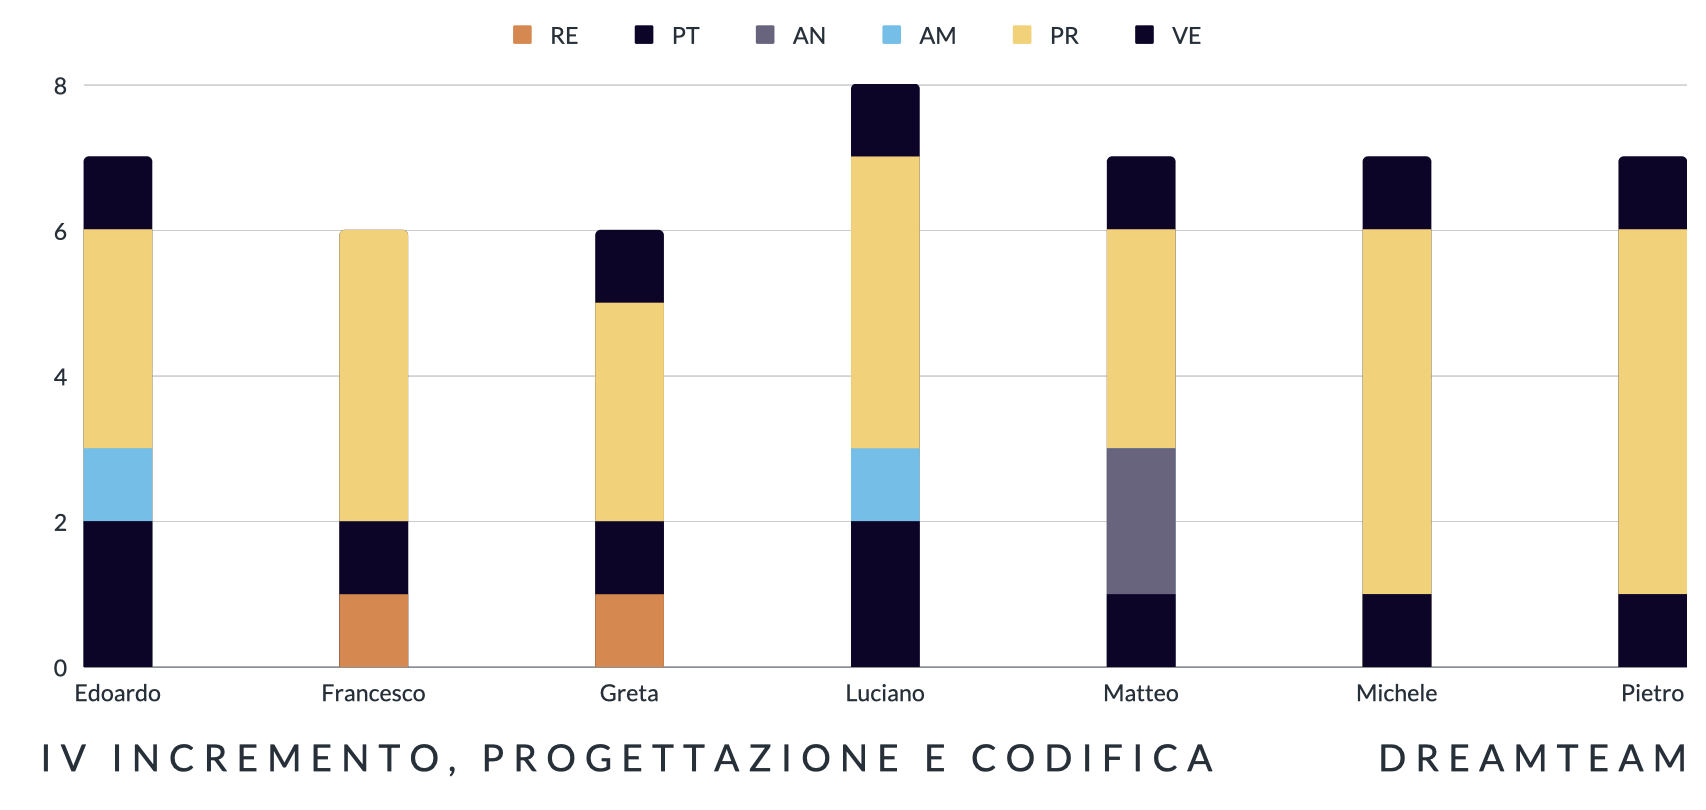
\includegraphics[scale=0.50]{Sezioni/SezioniPreventivo/grafici/progettazione/Progettazione_IV_incremento.png}
\caption{Istogramma della ripartizione delle ore nel IV incremento di Progettazione e Codifica}
\end{figure}

\subsubsubsection{Prospetto economico}
La seguente tabella rappresenta le ore totali dedicate ad ogni ruolo e il costo in euro:

\begin{table}[H]
\begin{center}
\rowcolors{2}{gray!25}{white}
\renewcommand{\arraystretch}{1.5}
\begin{tabular}{ m{0.3\textwidth}<{\centering}  m{0.2\textwidth}<{\centering} m{0.2\textwidth}<{\centering}}
	\rowcolor{darkblue}
	\textcolor{white}{\textbf{Ruolo}}&\textcolor{white}{\textbf{Totale ore}}&\textcolor{white}{\textbf{Costo totale (\euro)}}\\ 

	Responsabile  & 2 & 60 \\	
	
	Progettista & 9 & 225 \\
	
	Analista & 2 & 50 \\

	Amministratore & 2 & 40 \\
	
	Programmatore & 27 & 405 \\
	
	Verificatore & 6 & 90 \\
	
	\textbf{Totale} & 48 & 870 \\
	
\end{tabular}
\caption{Prospetto dei costi per ruolo nel IV incremento di Progettazione e Codifica}
\end{center}
\end{table}

La tabella può essere rappresentata anche in forma visiva dal seguente aerogramma:
\begin{figure}[H]
\centering
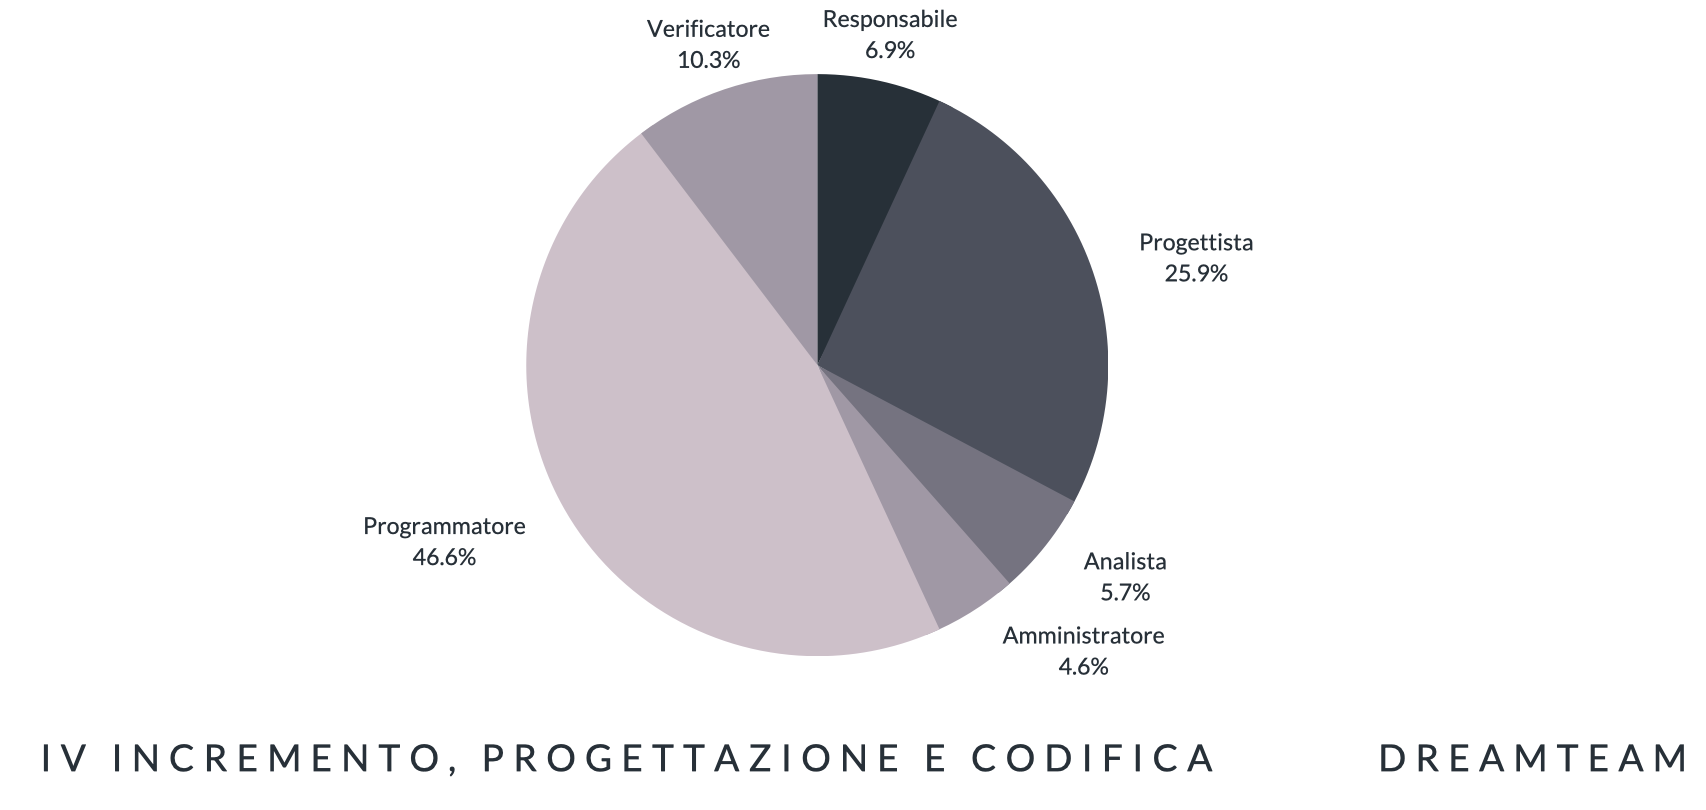
\includegraphics[scale=0.50]{Sezioni/SezioniPreventivo/grafici/progettazione/Progettazione_IV_incremento_costi.png}
\caption{Grafico a torta della ripartizione per ruolo delle ore durante il IV incremento di Progettazione e Codifica}
\end{figure}

\pagebreak

\subsubsection{V Incremento}
\subsubsubsection{Prospetto orario}
In questa fase la distribuzione oraria è la seguente:
\begin{table}[H]
\begin{center}
\rowcolors{2}{gray!25}{white}
\renewcommand{\arraystretch}{1.25}
\begin{tabular}{ m{0.20\textwidth}<{\centering}  m{0.06\textwidth}<{\centering} m{0.06\textwidth}<{\centering} m{0.06\textwidth}<{\centering}  m{0.06\textwidth}<{\centering}  m{0.06\textwidth}<{\centering}  m{0.06\textwidth}<{\centering}  m{0.20\textwidth}<{\centering}   }
	\rowcolor{darkblue}
	\textcolor{white}{\textbf{Componente}} &\textcolor{white}{\textbf{Re}}&\textcolor{white}{\textbf{Pt}}&\textcolor{white}{\textbf{An}}&\textcolor{white}{\textbf{Am}}&\textcolor{white}{\textbf{Pr}}&\textcolor{white}{\textbf{Ve}}&\textcolor{white}{\textbf{Ore complessive}}\\ 
	Edoardo Pavan & 0 & 2 & 0 & 1 & 3 & 1 & 7 \\	
	
	Francesco Protopapa & 0 & 1 & 0 & 0 & 4 & 1 & 6 \\

	Greta Cavedon & 0 & 0 & 0 & 0 & 2 & 1 & 3 \\
	
	Luciano Wu & 1 & 2 & 0 & 0 & 3 & 2 & 8 \\
	
	Matteo Basso & 0 & 1 & 1 & 0 & 3 & 1 & 6 \\
	
	Michele Gatto & 1 & 1 & 0 & 0 & 4 & 0 & 6 \\
	
	Pietro Villatora & 0 & 1 & 0 & 1 & 5 & 0 & 7 \\
	
	\textbf{Ore totali ruolo} & 2 & 8 & 1 & 2 & 24 & 6 & 43 \\

\end{tabular}
\caption{Distribuzione oraria per ogni componente nel V incremento di Progettazione e Codifica}
\end{center}
\end{table}

La tabella può essere rappresentata anche in forma visiva dal seguente grafico:
\begin{figure}[H]
\centering
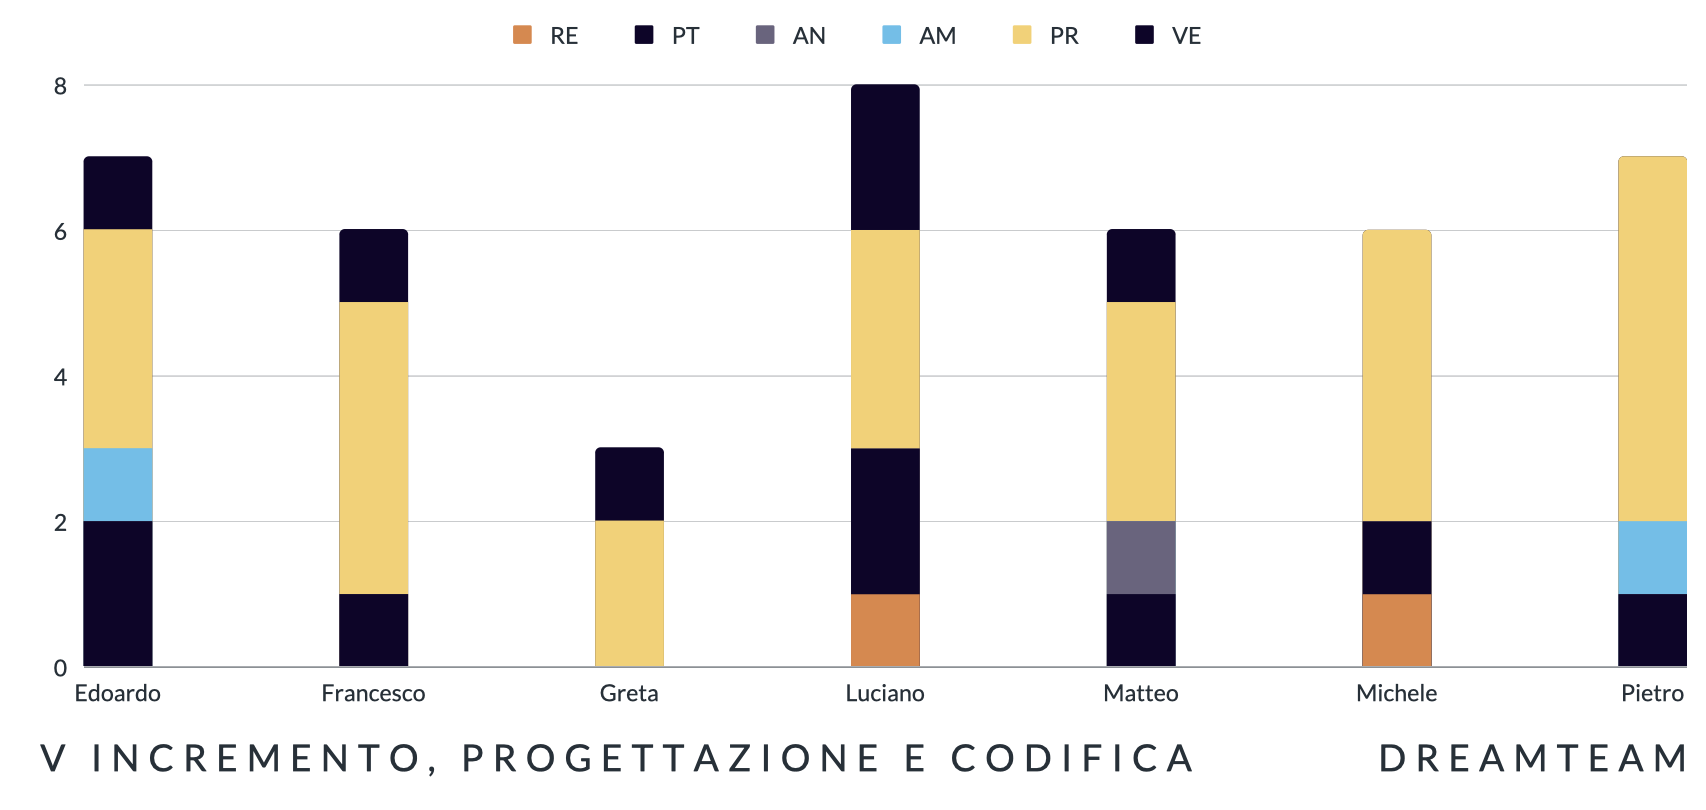
\includegraphics[scale=0.50]{Sezioni/SezioniPreventivo/grafici/progettazione/Progettazione_V_incremento.png}
\caption{Istogramma della ripartizione delle ore nel V incremento di Progettazione e Codifica}
\end{figure}

\subsubsubsection{Prospetto economico}
La seguente tabella rappresenta le ore totali dedicate ad ogni ruolo e il costo in euro:

\begin{table}[H]
\begin{center}
\rowcolors{2}{gray!25}{white}
\renewcommand{\arraystretch}{1.5}
\begin{tabular}{ m{0.3\textwidth}<{\centering}  m{0.2\textwidth}<{\centering} m{0.2\textwidth}<{\centering}}
	\rowcolor{darkblue}
	\textcolor{white}{\textbf{Ruolo}}&\textcolor{white}{\textbf{Totale ore}}&\textcolor{white}{\textbf{Costo totale (\euro)}}\\ 

	Responsabile & 2 & 60 \\	
	
	Progettista & 8 & 200 \\
	
	Analista & 1 & 25 \\

	Amministratore & 2 & 40 \\
	
	Programmatore & 24 & 360 \\
	
	Verificatore & 6 & 90 \\
	
	\textbf{Totale} & 43 & 775 \\
	
\end{tabular}
\caption{Prospetto dei costi per ruolo nel V incremento di Progettazione e Codifica}
\end{center}
\end{table}

La tabella può essere rappresentata anche in forma visiva dal seguente aerogramma:
\begin{figure}[H]
\centering
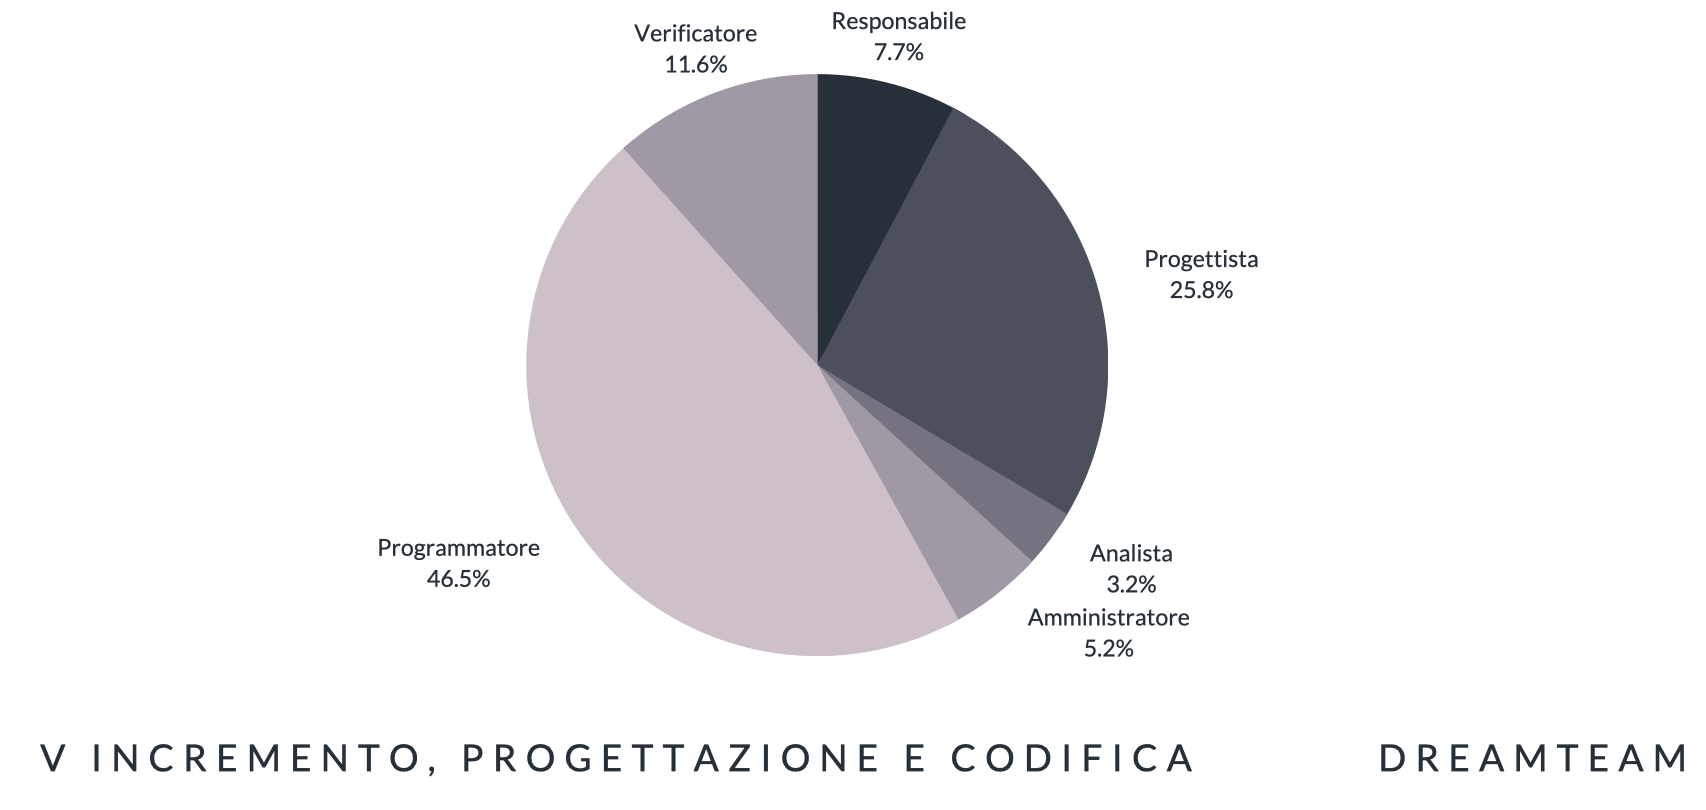
\includegraphics[scale=0.50]{Sezioni/SezioniPreventivo/grafici/progettazione/Progettazione_V_incremento_costi.png}
\caption{Grafico a torta della ripartizione per ruolo delle ore durante il V incremento di Progettazione e Codifica}
\end{figure}

\pagebreak


\subsubsection{VI Incremento}
\subsubsubsection{Prospetto orario}
In questa fase la distribuzione oraria è la seguente:
\begin{table}[H]
\begin{center}
\rowcolors{2}{gray!25}{white}
\renewcommand{\arraystretch}{1.25}
\begin{tabular}{ m{0.20\textwidth}<{\centering}  m{0.06\textwidth}<{\centering} m{0.06\textwidth}<{\centering} m{0.06\textwidth}<{\centering}  m{0.06\textwidth}<{\centering}  m{0.06\textwidth}<{\centering}  m{0.06\textwidth}<{\centering}  m{0.20\textwidth}<{\centering}   }
	\rowcolor{darkblue}
	\textcolor{white}{\textbf{Componente}} &\textcolor{white}{\textbf{Re}}&\textcolor{white}{\textbf{Pt}}&\textcolor{white}{\textbf{An}}&\textcolor{white}{\textbf{Am}}&\textcolor{white}{\textbf{Pr}}&\textcolor{white}{\textbf{Ve}}&\textcolor{white}{\textbf{Ore complessive}}\\ 
	Edoardo Pavan & 0 & 2 & 0 & 0 & 1 & 1 & 4 \\	
	
	Francesco Protopapa & 0 & 0 & 0 & 1 & 4 & 0 & 5 \\

	Greta Cavedon & 0 & 1 & 0 & 0 & 2 & 2 & 5 \\
	
	Luciano Wu & 1 & 1 & 0 & 0 & 3 & 1 & 6 \\
	
	Matteo Basso & 0 & 1 & 0 & 0 & 3 & 1 & 5 \\
	
	Michele Gatto & 1 & 2 & 0 & 0 & 4 & 0 & 7 \\
	
	Pietro Villatora & 0 & 1 & 0 & 0 & 5 & 1 & 7 \\
	
	\textbf{Ore totali ruolo} & 2 & 8 & 0 & 1 & 22 & 6 & 39 \\

\end{tabular}
\caption{Distribuzione oraria per ogni componente nel VI incremento di Progettazione e Codifica}
\end{center}
\end{table}

La tabella può essere rappresentata anche in forma visiva dal seguente grafico:
\begin{figure}[H]
\centering
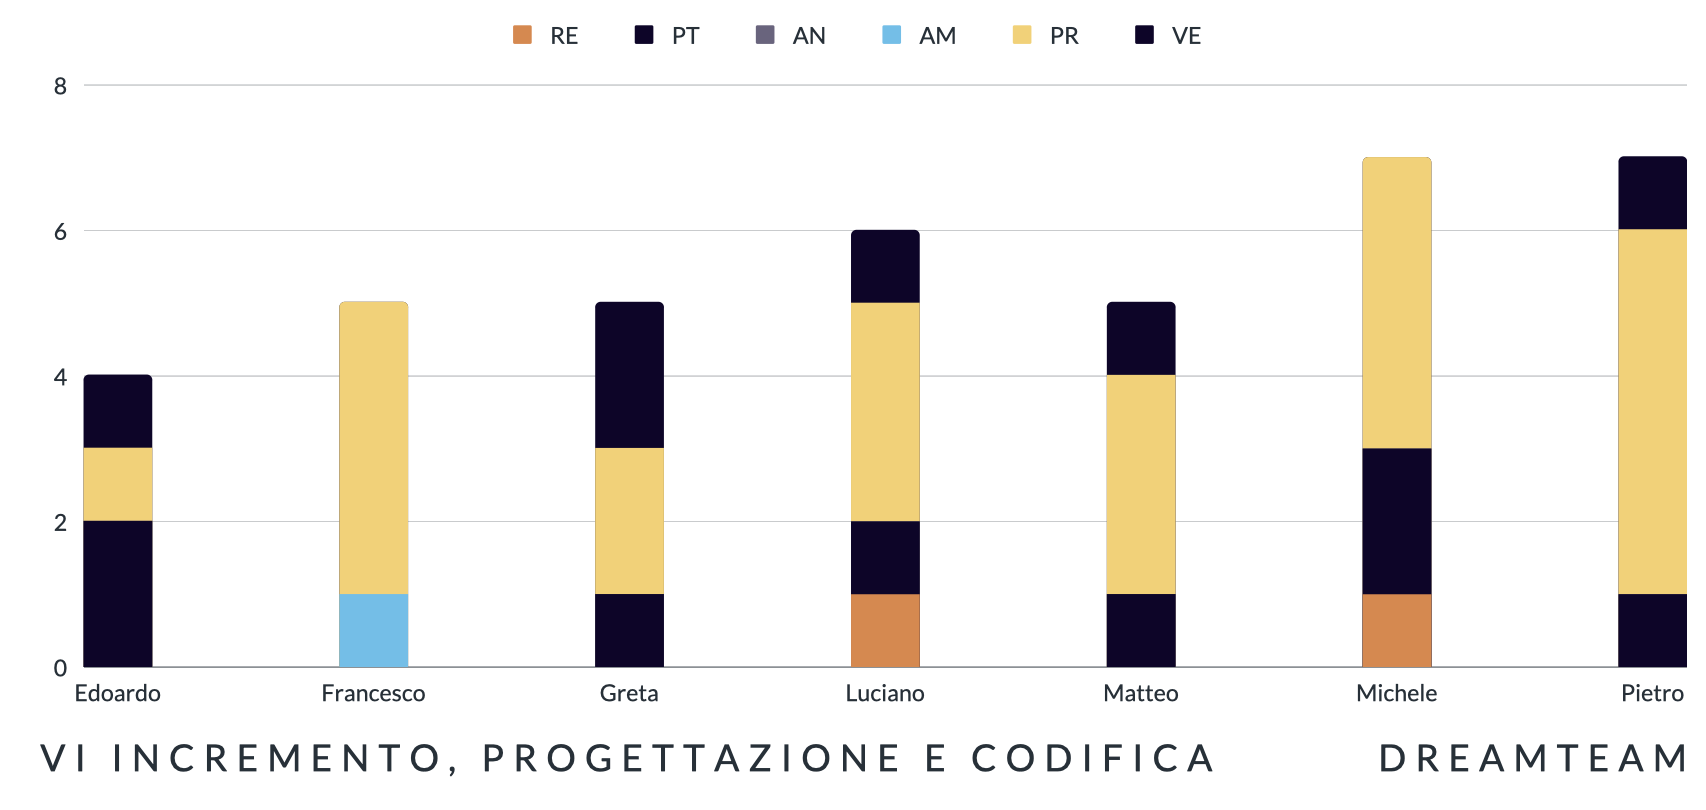
\includegraphics[scale=0.50]{Sezioni/SezioniPreventivo/grafici/progettazione/Progettazione_VI_incremento.png}
\caption{Istogramma della ripartizione delle ore nel VI incremento di Progettazione e Codifica}
\end{figure}

\subsubsubsection{Prospetto economico}
La seguente tabella rappresenta le ore totali dedicate ad ogni ruolo e il costo in euro:

\begin{table}[H]
\begin{center}
\rowcolors{2}{gray!25}{white}
\renewcommand{\arraystretch}{1.5}
\begin{tabular}{ m{0.3\textwidth}<{\centering}  m{0.2\textwidth}<{\centering} m{0.2\textwidth}<{\centering}}
	\rowcolor{darkblue}
	\textcolor{white}{\textbf{Ruolo}}&\textcolor{white}{\textbf{Totale ore}}&\textcolor{white}{\textbf{Costo totale (\euro)}}\\ 

	Responsabile  & 2 & 60 \\	
	
	Progettista & 8 & 200 \\
	
	Analista & 0 & 0 \\

	Amministratore & 1 & 20 \\
	
	Programmatore & 22 & 330 \\
	
	Verificatore & 6 & 90 \\
	
	\textbf{Totale} & 39 & 700 \\
	
\end{tabular}
\caption{Prospetto dei costi per ruolo nel VI incremento di Progettazione e Codifica}
\end{center}
\end{table}

La tabella può essere rappresentata anche in forma visiva dal seguente aerogramma:
\begin{figure}[H]
\centering
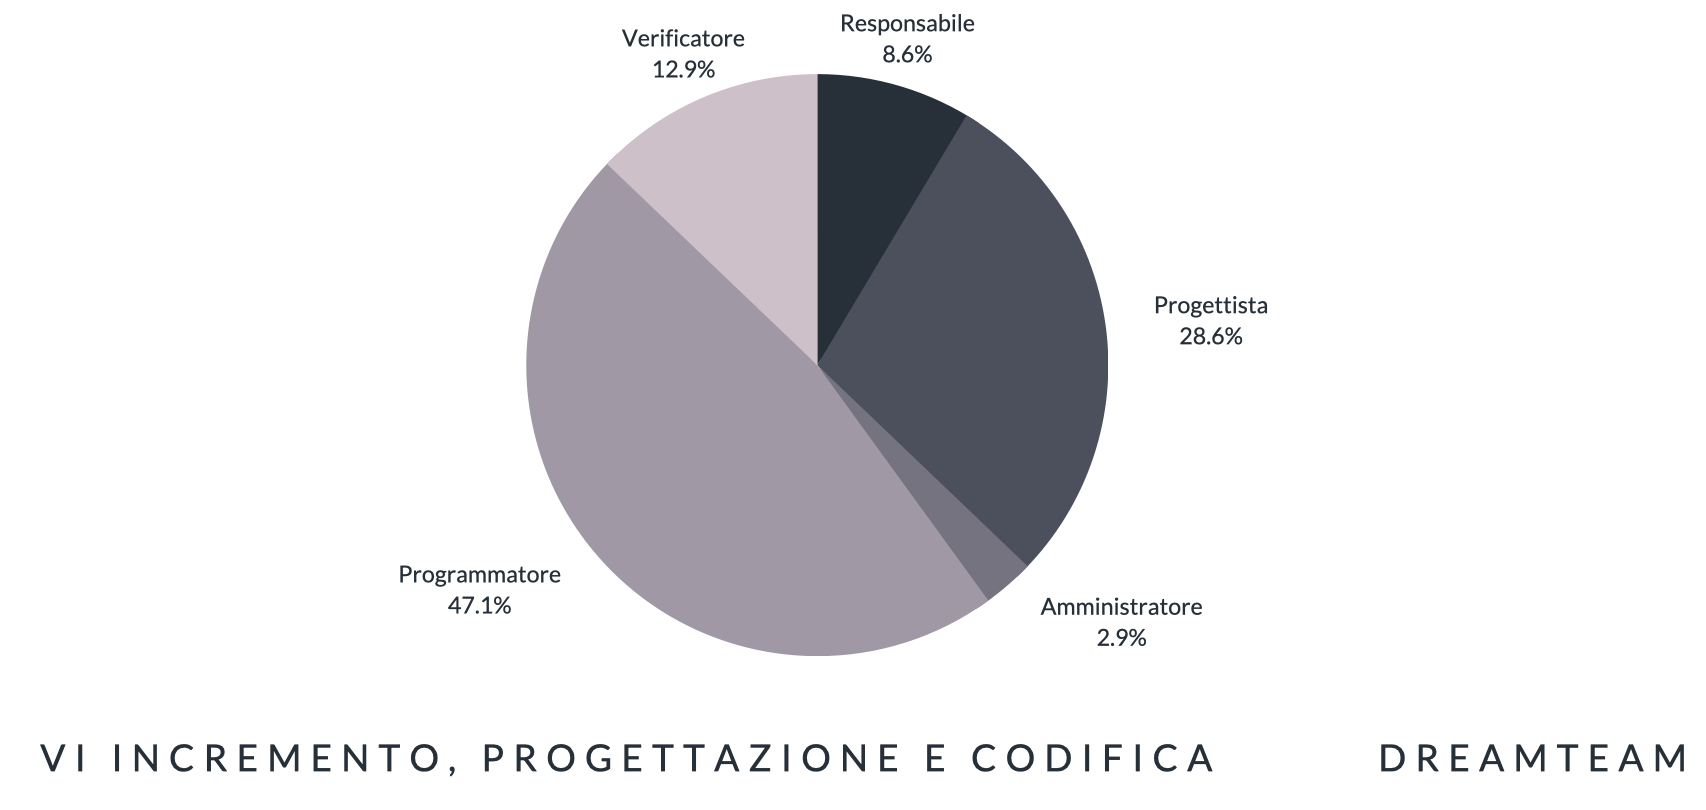
\includegraphics[scale=0.50]{Sezioni/SezioniPreventivo/grafici/progettazione/Progettazione_VI_incremento_costi.png}
\caption{Grafico a torta della ripartizione per ruolo delle ore durante il VI incremento di Progettazione e Codifica}
\end{figure}

\pagebreak


\subsubsection{VII Incremento}
\subsubsubsection{Prospetto orario}
In questa fase la distribuzione oraria è la seguente:
\begin{table}[H]
\begin{center}
\rowcolors{2}{gray!25}{white}
\renewcommand{\arraystretch}{1.25}
\begin{tabular}{ m{0.20\textwidth}<{\centering}  m{0.06\textwidth}<{\centering} m{0.06\textwidth}<{\centering} m{0.06\textwidth}<{\centering}  m{0.06\textwidth}<{\centering}  m{0.06\textwidth}<{\centering}  m{0.06\textwidth}<{\centering}  m{0.20\textwidth}<{\centering}   }
	\rowcolor{darkblue}
	\textcolor{white}{\textbf{Componente}} &\textcolor{white}{\textbf{Re}}&\textcolor{white}{\textbf{Pt}}&\textcolor{white}{\textbf{An}}&\textcolor{white}{\textbf{Am}}&\textcolor{white}{\textbf{Pr}}&\textcolor{white}{\textbf{Ve}}&\textcolor{white}{\textbf{Ore complessive}}\\ 
	Edoardo Pavan & 0 & 2 & 0 & 0 & 0 & 1 & 3 \\	
	
	Francesco Protopapa & 0 & 1 & 0 & 0 & 2 & 0 & 3 \\

	Greta Cavedon & 1 & 1 & 0 & 0 & 2 & 1 & 5 \\
	
	Luciano Wu & 0 & 1 & 0 & 1 & 3 & 1 & 6 \\
	
	Matteo Basso & 0 & 0 & 0 & 0 & 3 & 1 & 4 \\
	
	Michele Gatto & 0 & 1 & 0 & 0 & 4 & 0 & 5 \\
	
	Pietro Villatora & 0 & 0 & 0 & 0 & 5 & 1 & 6 \\
	
	\textbf{Ore totali ruolo} & 1 & 6 & 0 & 1 & 19 & 5 & 32 \\

\end{tabular}
\caption{Distribuzione oraria per ogni componente nel VII incremento di Progettazione e Codifica}
\end{center}
\end{table}

La tabella può essere rappresentata anche in forma visiva dal seguente grafico:
\begin{figure}[H]
\centering
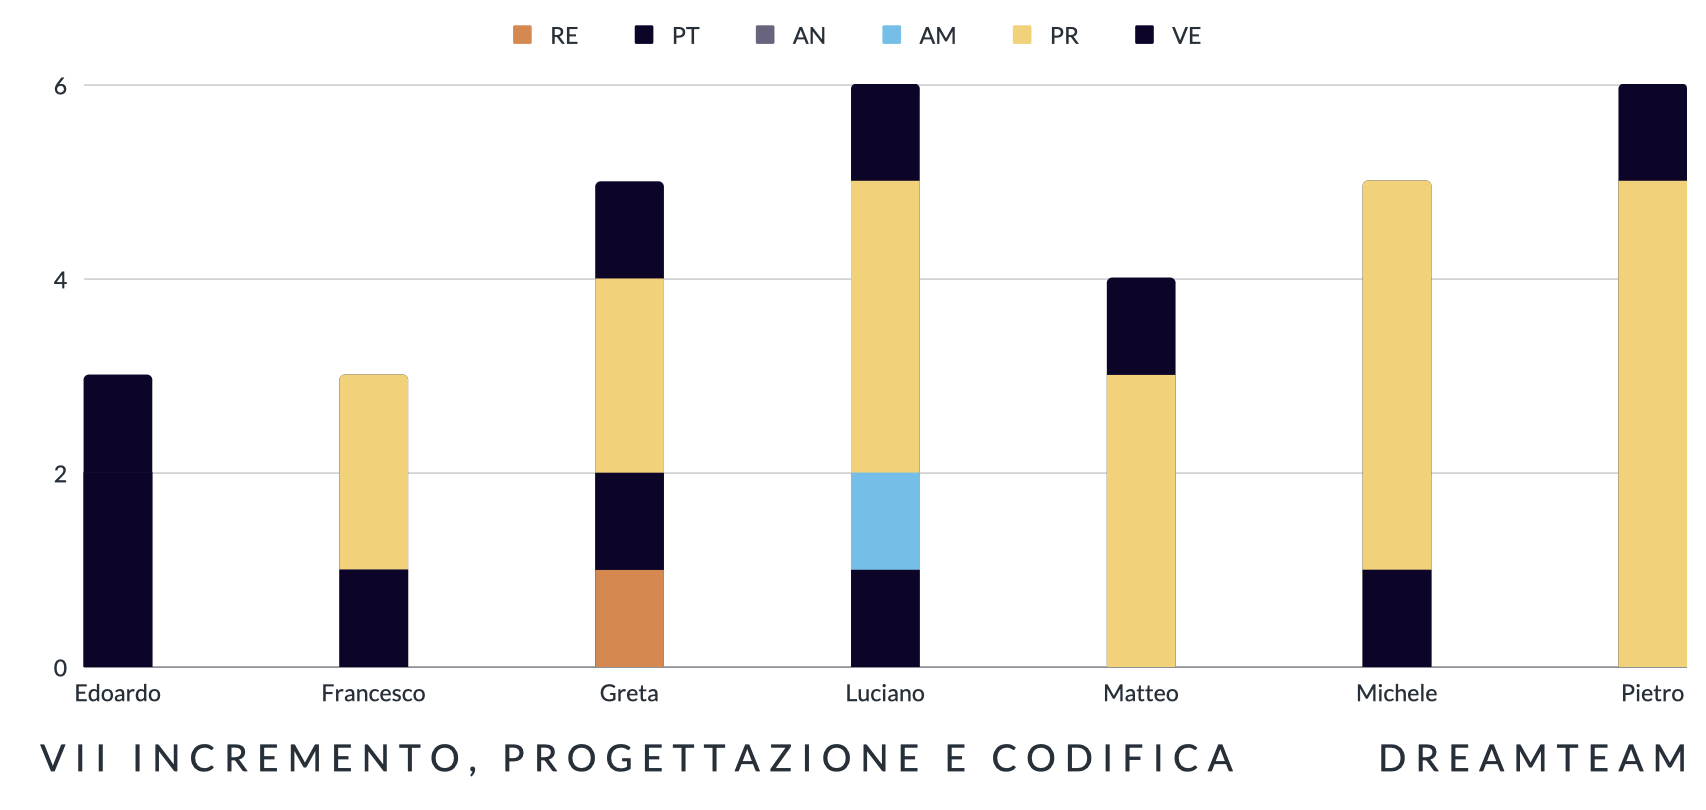
\includegraphics[scale=0.0]{Sezioni/SezioniPreventivo/grafici/progettazione/Progettazione_VII_incremento.png}
\caption{Istogramma della ripartizione delle ore nel VII incremento di Progettazione e Codifica}
\end{figure}

\subsubsubsection{Prospetto economico}
La seguente tabella rappresenta le ore totali dedicate ad ogni ruolo e il costo in euro:

\begin{table}[H]
\begin{center}
\rowcolors{2}{gray!25}{white}
\renewcommand{\arraystretch}{1.5}
\begin{tabular}{ m{0.3\textwidth}<{\centering}  m{0.2\textwidth}<{\centering} m{0.2\textwidth}<{\centering}}
	\rowcolor{darkblue}
	\textcolor{white}{\textbf{Ruolo}}&\textcolor{white}{\textbf{Totale ore}}&\textcolor{white}{\textbf{Costo totale (\euro)}}\\ 

	Responsabile  & 1 & 30 \\	
	
	Progettista & 6 & 150 \\
	
	Analista & 0 & 0 \\

	Amministratore & 1 & 20 \\
	
	Programmatore & 19 & 285 \\
	
	Verificatore & 5 & 75 \\
	
	\textbf{Totale} & 32 & 560 \\
	
\end{tabular}
\caption{Prospetto dei costi per ruolo nel VII incremento di Progettazione e Codifica}
\end{center}
\end{table}

La tabella può essere rappresentata anche in forma visiva dal seguente aerogramma:
\begin{figure}[H]
\centering
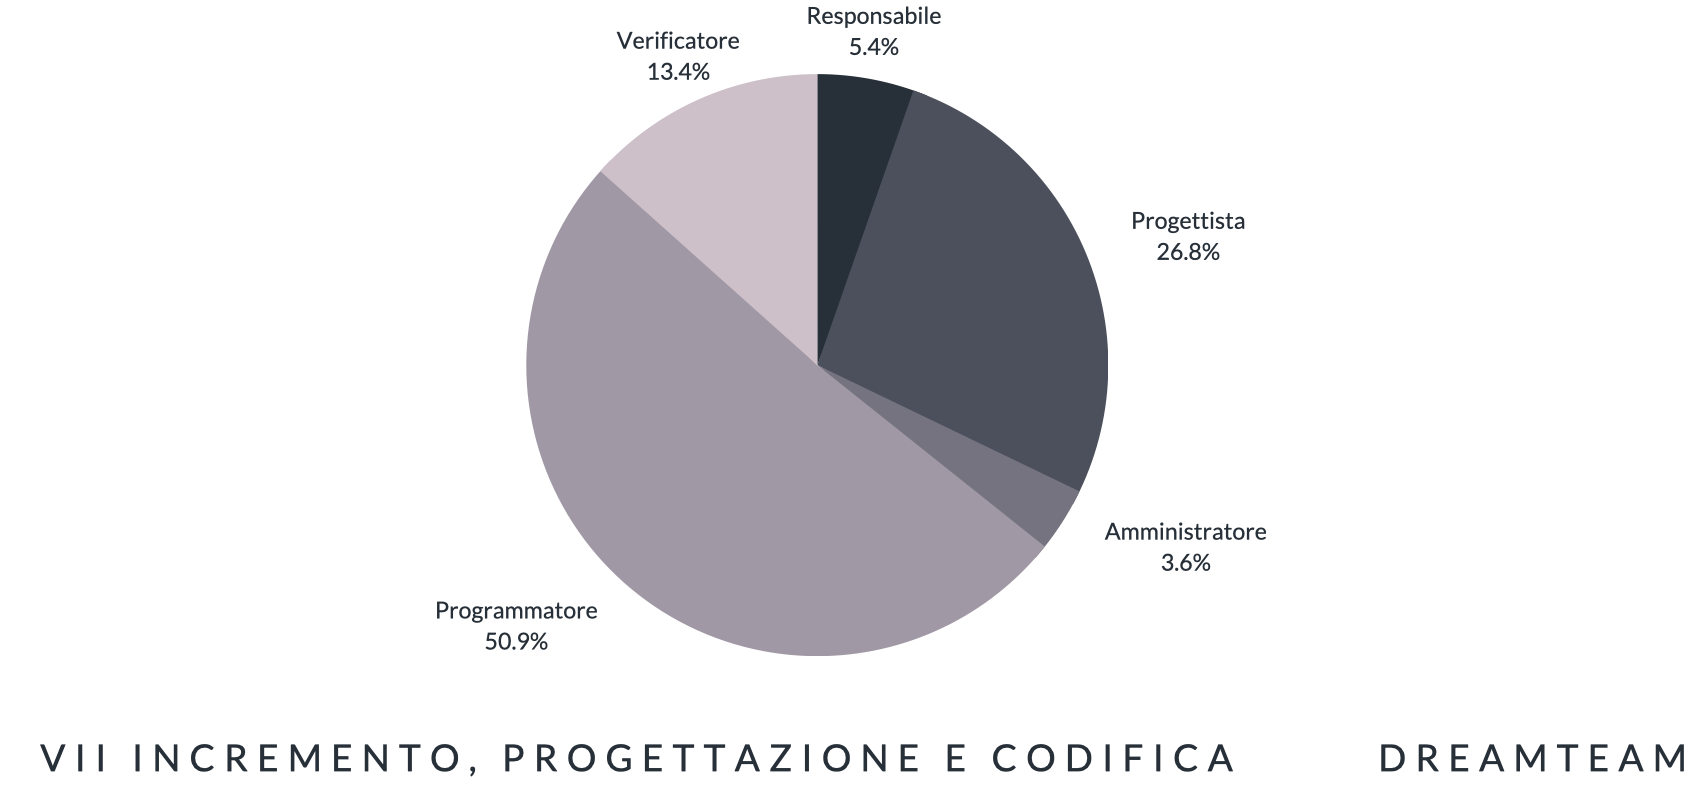
\includegraphics[scale=0.50]{Sezioni/SezioniPreventivo/grafici/progettazione/Progettazione_VII_incremento_costi.png}
\caption{Grafico a torta della ripartizione per ruolo delle ore durante il VII incremento di Progettazione e Codifica}
\end{figure}

\pagebreak


\subsubsection{VIII Incremento}
\subsubsubsection{Prospetto orario}
In questa fase la distribuzione oraria è la seguente:
\begin{table}[H]
\begin{center}
\rowcolors{2}{gray!25}{white}
\renewcommand{\arraystretch}{1.25}
\begin{tabular}{ m{0.20\textwidth}<{\centering}  m{0.06\textwidth}<{\centering} m{0.06\textwidth}<{\centering} m{0.06\textwidth}<{\centering}  m{0.06\textwidth}<{\centering}  m{0.06\textwidth}<{\centering}  m{0.06\textwidth}<{\centering}  m{0.20\textwidth}<{\centering}   }
	\rowcolor{darkblue}
	\textcolor{white}{\textbf{Componente}} &\textcolor{white}{\textbf{Re}}&\textcolor{white}{\textbf{Pt}}&\textcolor{white}{\textbf{An}}&\textcolor{white}{\textbf{Am}}&\textcolor{white}{\textbf{Pr}}&\textcolor{white}{\textbf{Ve}}&\textcolor{white}{\textbf{Ore complessive}}\\ 
	Edoardo Pavan & 0 & 0 & 0 & 0 & 0 & 2 & 2 \\	
	
	Francesco Protopapa & 0 & 1 & 0 & 0 & 2 & 1 & 4 \\

	Greta Cavedon & 0 & 1 & 0 & 0 & 0 & 2 & 3 \\
	
	Luciano Wu & 1 & 0 & 0 & 1 & 3 & 0 & 5 \\
	
	Matteo Basso & 0 & 1 & 0 & 0 & 3 & 0 & 4 \\
	
	Michele Gatto & 0 & 1 & 0 & 0 & 3 & 0 & 4 \\
	
	Pietro Villatora & 0 & 1 & 0 & 0 & 1 & 1 & 3 \\
	
	\textbf{Ore totali ruolo} & 2 & 4 & 0 & 1 & 12 & 6 & 25 \\

\end{tabular}
\caption{Distribuzione oraria per ogni componente nel VIII incremento di Progettazione e Codifica}
\end{center}
\end{table}

La tabella può essere rappresentata anche in forma visiva dal seguente grafico:
\begin{figure}[H]
\centering
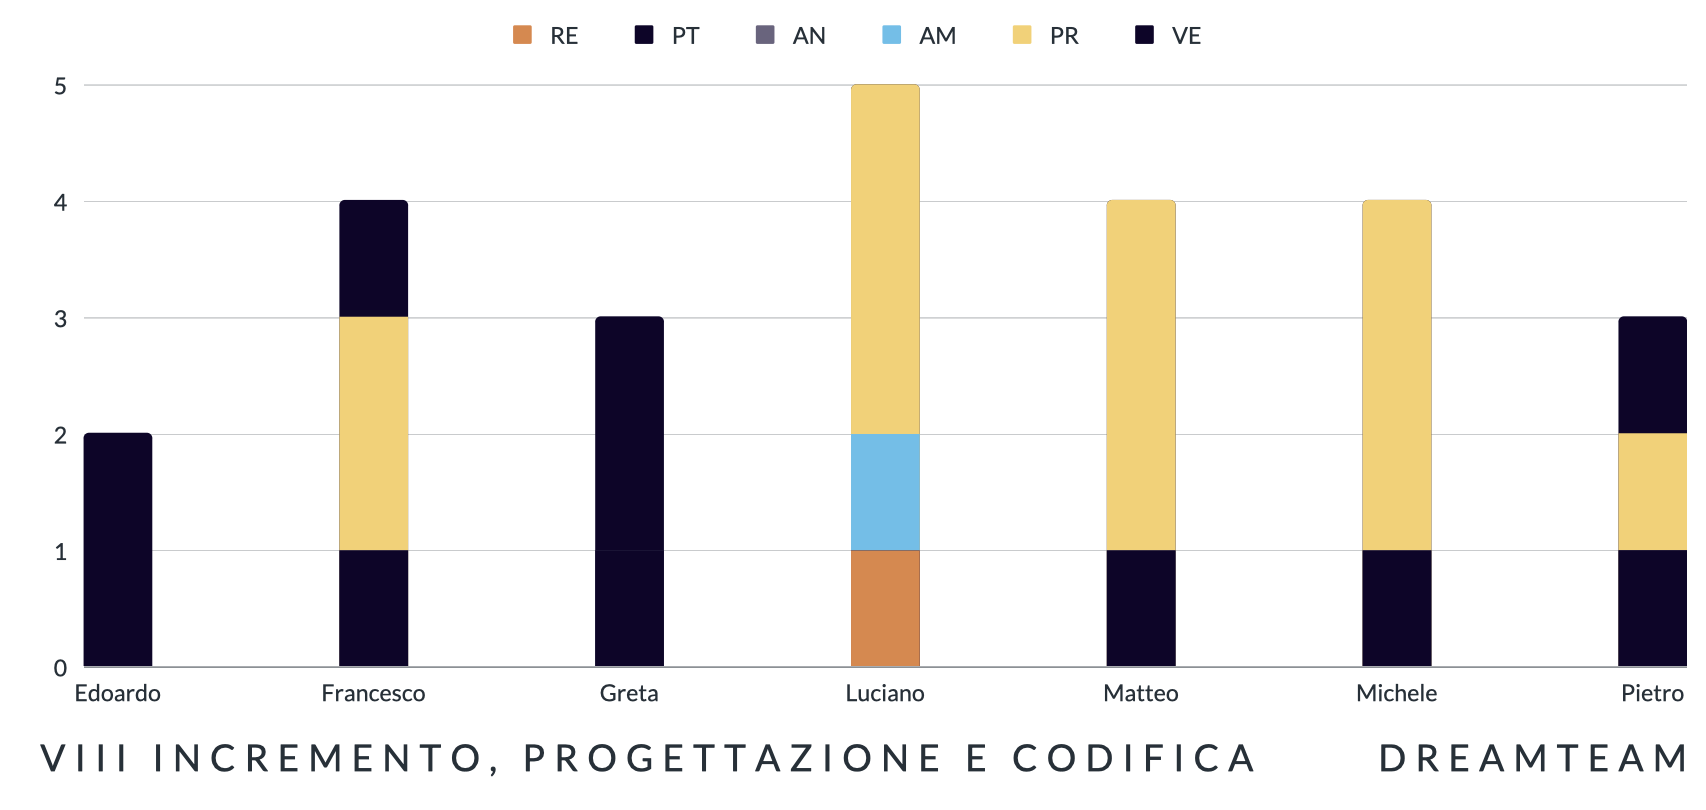
\includegraphics[scale=0.50]{Sezioni/SezioniPreventivo/grafici/progettazione/Progettazione_VIII_incremento.png}
\caption{Istogramma della ripartizione delle ore nel VIII incremento di Progettazione e Codifica}
\end{figure}

\subsubsubsection{Prospetto economico}
La seguente tabella rappresenta le ore totali dedicate ad ogni ruolo e il costo in euro:

\begin{table}[H]
\begin{center}
\rowcolors{2}{gray!25}{white}
\renewcommand{\arraystretch}{1.5}
\begin{tabular}{ m{0.3\textwidth}<{\centering}  m{0.2\textwidth}<{\centering} m{0.2\textwidth}<{\centering}}
	\rowcolor{darkblue}
	\textcolor{white}{\textbf{Ruolo}}&\textcolor{white}{\textbf{Totale ore}}&\textcolor{white}{\textbf{Costo totale (\euro)}}\\ 

	Responsabile  & 2 & 60 \\	
	
	Progettista & 4 & 100 \\
	
	Analista & 0 & 0 \\

	Amministratore & 1 & 20 \\
	
	Programmatore & 12 & 180 \\
	
	Verificatore & 6 & 90 \\
	
	\textbf{Totale} & 25 & 450 \\
	
\end{tabular}
\caption{Prospetto dei costi per ruolo nel VIII incremento di Progettazione e Codifica}
\end{center}
\end{table}

La tabella può essere rappresentata anche in forma visiva dal seguente aerogramma:
\begin{figure}[H]
\centering
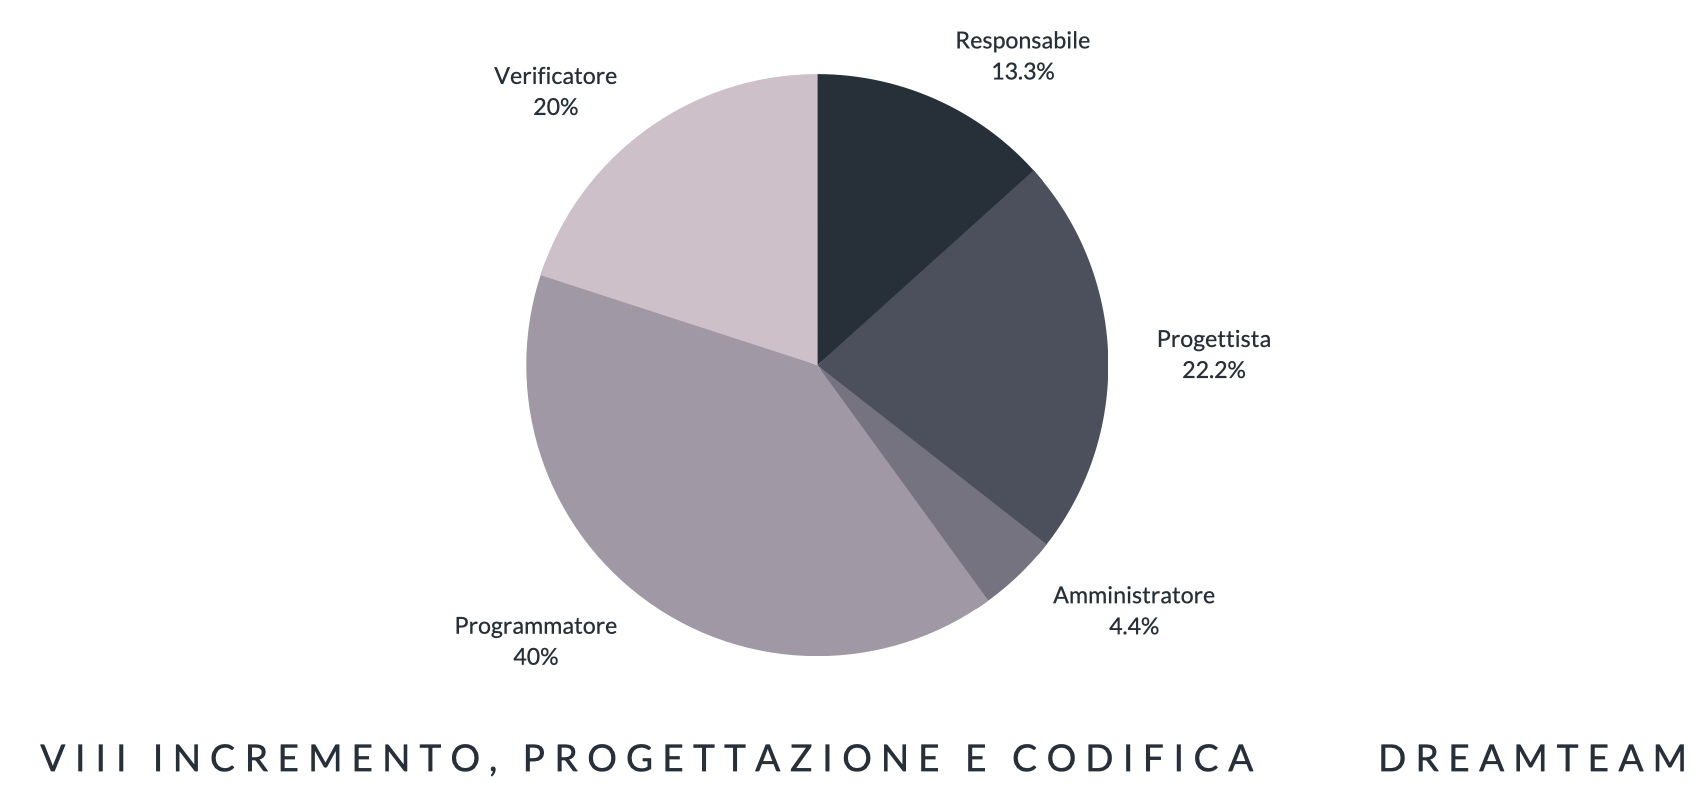
\includegraphics[scale=0.50]{Sezioni/SezioniPreventivo/grafici/progettazione/Progettazione_VIII_incremento_costi.png}
\caption{Grafico a torta della ripartizione per ruolo delle ore durante il VIII incremento di Progettazione e Codifica}
\end{figure}

\pagebreak


\subsubsection{Fase complessiva}
\subsubsubsection{Prospetto orario}
La seguente tabella rappresenta la distribuzione oraria per ogni componente del gruppo nella fase di progettazione e codifica:
\begin{table}[H]
\begin{center}
\rowcolors{2}{gray!25}{white}
\renewcommand{\arraystretch}{1.25}
\begin{tabular}{ m{0.20\textwidth}<{\centering}  m{0.06\textwidth}<{\centering} m{0.06\textwidth}<{\centering} m{0.06\textwidth}<{\centering}  m{0.06\textwidth}<{\centering}  m{0.06\textwidth}<{\centering}  m{0.06\textwidth}<{\centering}  m{0.20\textwidth}<{\centering}   }
	\rowcolor{darkblue}
	\textcolor{white}{\textbf{Componente}} &\textcolor{white}{\textbf{Re}}&\textcolor{white}{\textbf{Pt}}&\textcolor{white}{\textbf{An}}&\textcolor{white}{\textbf{Am}}&\textcolor{white}{\textbf{Pr}}&\textcolor{white}{\textbf{Ve}}&\textcolor{white}{\textbf{Ore complessive}}\\ 
	Edoardo Pavan & 2 & 13 & 0 & 5 & 13 & 10 & 43 \\	
	
	Francesco Protopapa & 2 & 8 & 0 & 1 & 20 & 6 & 37 \\

	Greta Cavedon & 3 & 7 & 0 & 0 & 16 & 10 & 36 \\
	
	Luciano Wu & 5 & 10 & 0 & 5 & 23 & 6 & 49 \\
	
	Matteo Basso & 0 & 9 & 7 & 0 & 25 & 7 & 48 \\
	
	Michele Gatto & 6 & 8 & 0 & 0 & 27 & 5 & 46 \\
	
	Pietro Villatora & 0 & 8 & 0 & 2 & 31 & 6 & 47 \\
	
	\textbf{Ore totali ruolo} & 18 & 63 & 7 & 13 & 155 & 50 & 306\\

\end{tabular}
\caption{Distribuzione oraria per ogni componente nella fase di Progettazione e Codifica}
\end{center}
\end{table}

La tabella può essere rappresentata anche in forma visiva dal seguente grafico:
\begin{figure}[H]
\centering
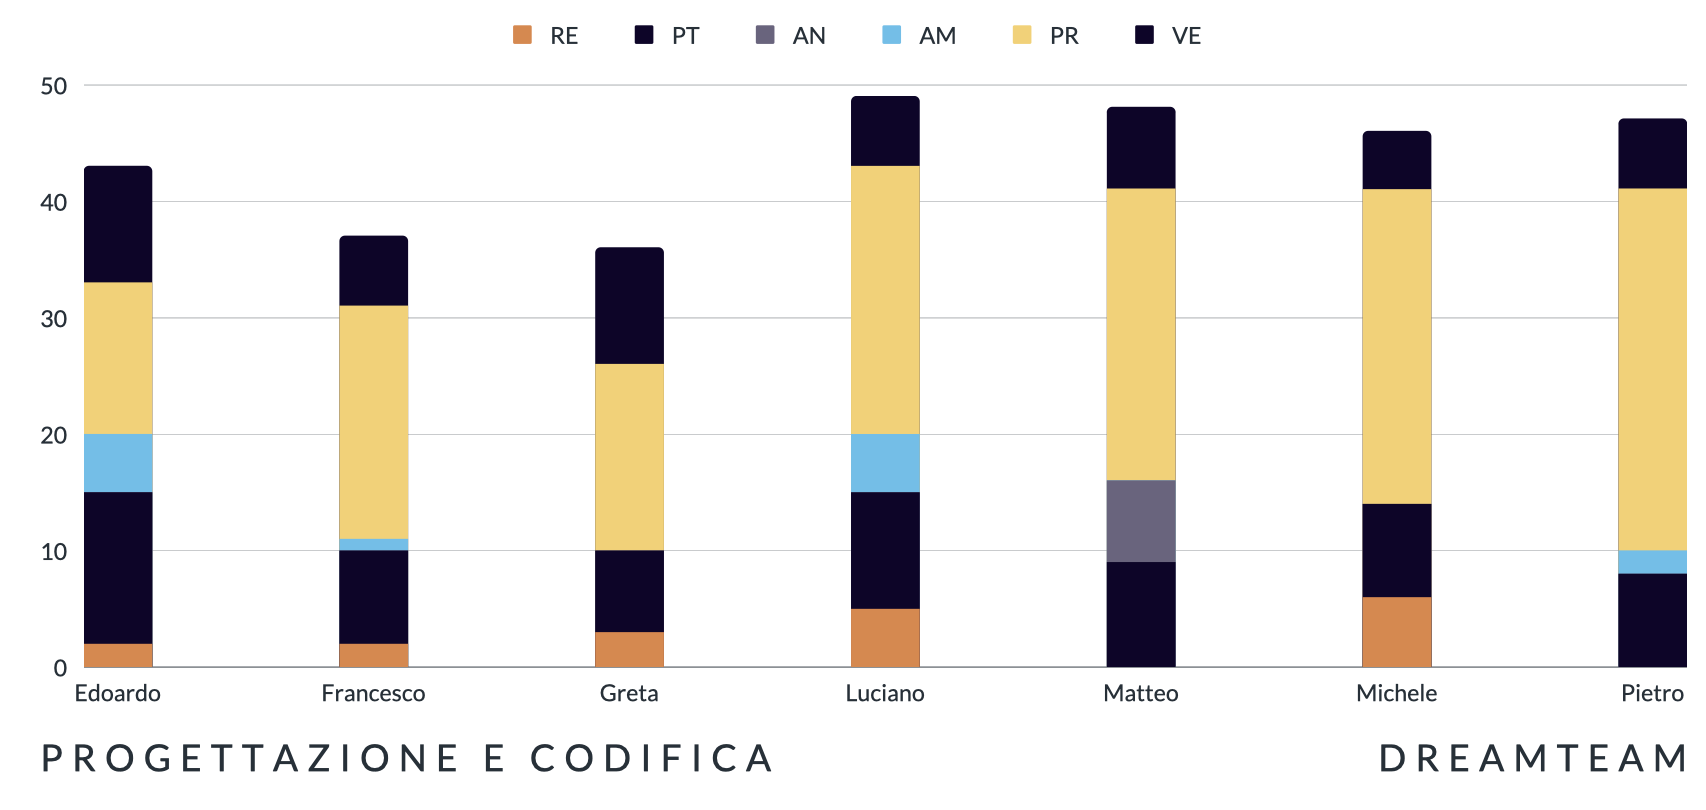
\includegraphics[scale=0.50]{Sezioni/SezioniPreventivo/grafici/progettazione/Progettazione.png}
\caption{Istogramma della ripartizione delle ore nella fase di Progettazione e Codifica}
\end{figure}

\subsubsubsection{Prospetto economico}
La seguente tabella rappresenta le ore totali dedicate ad ogni ruolo e il costo in euro:

\begin{table}[H]
\begin{center}
\rowcolors{2}{gray!25}{white}
\renewcommand{\arraystretch}{1.5}
\begin{tabular}{ m{0.3\textwidth}<{\centering}  m{0.2\textwidth}<{\centering} m{0.2\textwidth}<{\centering}}
	\rowcolor{darkblue}
	\textcolor{white}{\textbf{Ruolo}}&\textcolor{white}{\textbf{Totale ore}}&\textcolor{white}{\textbf{Costo totale (\euro)}}\\ 

	Responsabile & 18 & 540 \\	
	
	Progettista & 63 & 1575 \\
	
	Analista & 7 & 175 \\

	Amministratore & 13 & 260 \\
	
	Programmatore & 155 & 2325 \\
	
	Verificatore & 50 & 750 \\
	
	\textbf{Totale} & 306 & 5625 \\
	
\end{tabular}
\caption{Prospetto dei costi per ruolo nella fase di Progettazione e Codifica}
\end{center}
\end{table}

La tabella può essere rappresentata anche in forma visiva dal seguente aerogramma:
\begin{figure}[H]
\centering
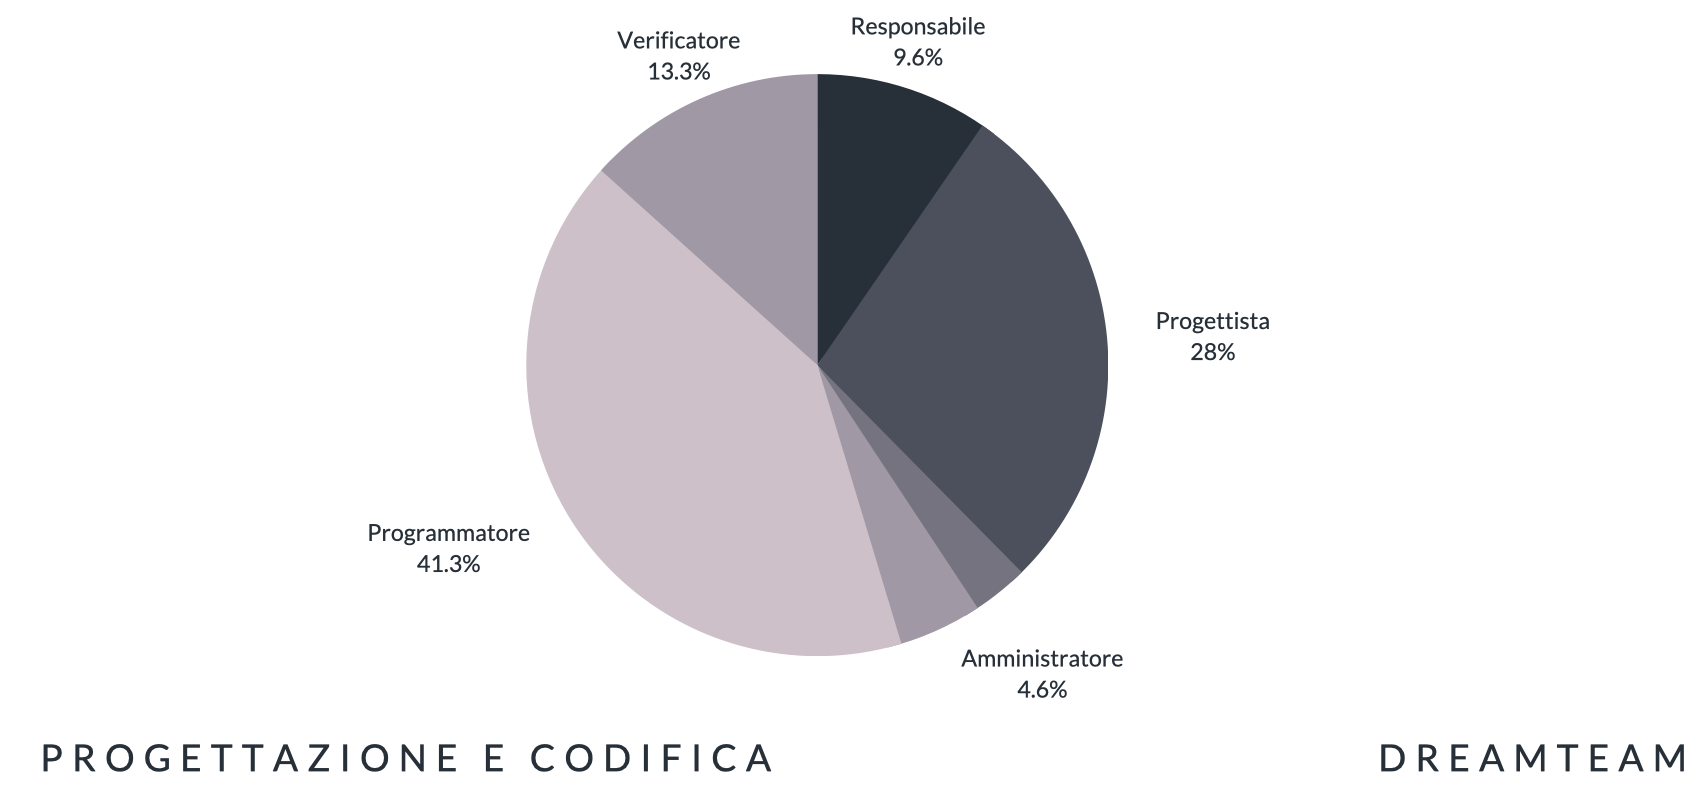
\includegraphics[scale=0.50]{Sezioni/SezioniPreventivo/grafici/progettazione/Progettazione_costi.png}
\caption{Grafico a torta della ripartizione per ruolo delle ore durante la fase di Progettazione e Codifica}
\end{figure}



